\documentclass[11pt, a4paper]{article}
\usepackage[T2A]{fontenc}
\usepackage[utf8]{inputenc}
\usepackage[serbianc]{babel}
\usepackage[left=2.5cm, top=1.75cm, bottom=1.5cm, right=1cm]{geometry}
\usepackage{graphicx}
\usepackage{fontspec}
\usepackage{enumerate}
\usepackage[export]{adjustbox}
\usepackage{textcomp}
\usepackage{array}
\usepackage{amsmath}
\usepackage{amssymb}
\usepackage{gensymb}
\usepackage{pdfpages}
\usepackage{hyperref}
\usepackage{fancyhdr}
\usepackage{subcaption}
\usepackage{mwe}
\usepackage{float}
\usepackage{listings}
\usepackage{color}
%KOD
\definecolor{dkgreen}{rgb}{0,0.6,0}
\definecolor{gray}{rgb}{0.5,0.5,0.5}
\definecolor{mauve}{rgb}{0.58,0,0.82}

\lstset{frame=tb,
  language=Python,
  aboveskip=3mm,
  belowskip=3mm,
  showstringspaces=false,
  columns=flexible,
  basicstyle={\small\ttfamily},
  numbers=none,
  numberstyle=\tiny\color{gray},
  keywordstyle=\color{blue},
  commentstyle=\color{dkgreen},
  stringstyle=\color{mauve},
  breaklines=true,
  breakatwhitespace=true,
  tabsize=3
}

%REFERENCE
\usepackage[nottoc]{tocbibind}
\usepackage[backend=biber]{biblatex}
\addbibresource{Reference.bib}
\renewcommand*{\thesection}{\arabic{section}}
\hypersetup{
    colorlinks=true,
    linkcolor=blue,
    filecolor=magenta,      
    urlcolor=cyan,
}
\setmainfont{Ubuntu Light}
\pagestyle{fancy}
\fancyhf{}
\fancyhead[R]{Виши курс методе коначних елемената}
\fancyhead[L]{Синтезни рад}
\fancyhead[C]{%
\ifnum\value{part}>0 \partname \ \thepart \fi}

\rfoot{Страна \thepage}
\fancyfoot[CE,LO]{\leftmark}

%PARAGRAF podesavanja
\setlength{\parskip}{1.5mm}
\setlength{\parindent}{0mm}

\begin{document}

\thispagestyle{empty}
\setcounter{tocdepth}{2}
\thispagestyle{empty}
\title{\vspace{-1cm} Универзитет у Београду\\ Грађевински факултет}
%\author{\Large{Пројекат армиранобетонске конструкције вишеспратне стамбено пословне зграде}}
\date{\vspace{-5ex}}
%\date{@}
\maketitle
\begin{center}

\includegraphics[scale=1]{Slike/Grb.png}
\end{center}
 
\begin{center}
\Huge {Семинарски рад}
\end{center}
\vspace{1cm}
\begin{center}
\huge{Виши курс методе коначних елемената}
\end{center}
\vspace{3cm}

\Large{Студенти:
\hfill
Ментори:
\par
Вукашин Томановић 588/20
\hfill
др. Марија T. Нефовска-Даниловић\\
Јован Пантовић 638/20
\hfill
др. Мирослав Маријановић\\
Никола Лакић 641/20 \\
Рајко Бабић 639/20
  }

\thispagestyle{empty}
\newpage

\tableofcontents{}
\thispagestyle{empty}
\newpage
\setcounter{page}{1}
\section{Увод}
\subsection{Принцип методе коначних елемената} 
Метода коначних елемената представља методу нумеричког решавања диференцијалних једначина са граничним условима којима је описан физички дискретизован модел. Дискретизација модела се врши коначним елементима.
\par
Коначни елемент је мали (геометријски) део континуума модела (плоча, греда, љуска итд) који је део мреже коначних елемената које дискретизују континуум. У једном коначном елементу су дефинисани чворови чији број и распоред зависи од типа коначног елемента, а у чворовима се дефинишу основне непознате које са интерполационим функцијама $N$ дефинишу поље непознатих.  Локални координатни систем коначног елемента може бити глобални $(x,y)$ или изопараметарски $(\xi, \eta)$. Пример за коначни елемент типа $Q9$  где су за основне непознате усвојена померања којих има два по чвору (укупно 18) , померања $x_i$ су у $X$ правцу док су $y_i$ у $Y$ правцу:

\begin{eqnarray}
	x(x,y) = \sum_{i=1}^9N_i \cdot x_i \\
	y(x,y) = \sum_{i=1}^9N_i \cdot y_i 
\end{eqnarray}

Као познате се узимају гранични услови у чворовима коначног елемента који у општем случају могу бити дати по померањима, силама или мешовито.\\
Неки типови коначних елемената, за непознате у чворовима су на сликама усвојена померања:
\begin{figure}[H]
	\subcaptionbox{Линеарни КЕ са два чвора}{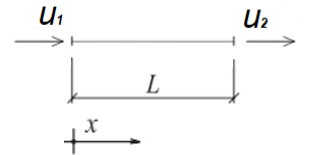
\includegraphics[width=0.22\textwidth]{Slike/Linear2node.png}} \hfill
	\subcaptionbox{CST коначни елемент}{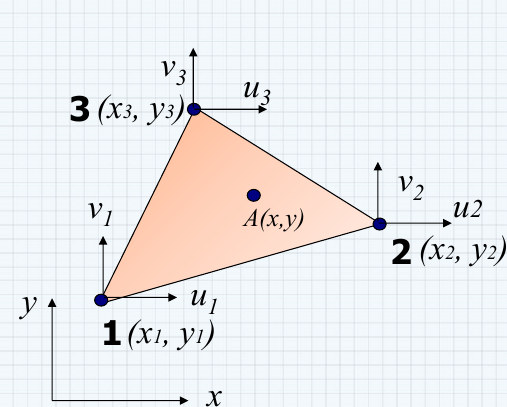
\includegraphics[width=0.22\textwidth]{Slike/CST_slika.png}}\hfill
	\subcaptionbox{Q4 коначни елемент}{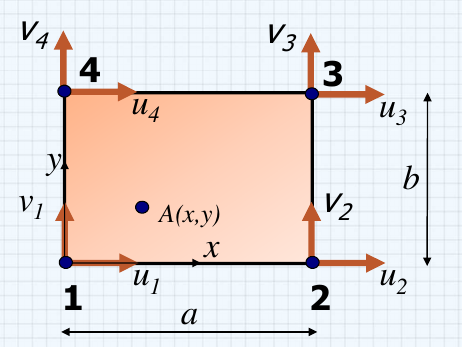
\includegraphics[width=0.22\textwidth]{Slike/Q4.png}} \hfill
	\subcaptionbox{Q9 коначни елемент }{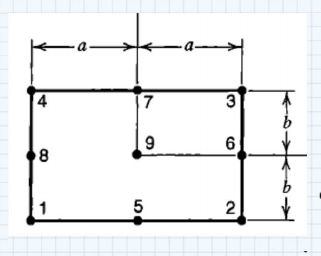
\includegraphics[width=0.22\textwidth]{Slike/Q9.png}} \hfill
	\caption{Типови коначних елемената \cite{mnd1}}
	\end{figure}
\par 
Интерполационе функције $N_i$ су дефинисане као функције чија је вредност у тачки посматраног чвора једнака јединици док је у тачкама осталих чворова та вредност једнака нули. За интерполационе функције се бирају полиноми чији ред зависи од типа коначног елемента. Полиноми се бирају из разлога лакше диференцијације и интеграције. Пример интерполационе функције $N_9$ за равански коначни елемент са девет чвора (Q9) у изопараметарском координатном систему:
\begin{eqnarray}
	N_9 &=& (1-\xi ^2)(1- \eta ^2)
\end{eqnarray}
\par
У чворовима коначних елемената се налазе непознате/познате које од зависности од типа коначног елемента чине уређене н-торке. Обично се за основне непознате коначог елемента узимају генералисана померања јер се њиховим одређивањем лако долази до пресечних сила преко матрице крутости уз помоћ познатог израза:
\begin{eqnarray}
	\mathbb{R} = \mathbb{K} \cdot q
\end{eqnarray}

Даље уз помоћ одређених парцијалних диференцијала поља померања одређујемо и  напонско стање унутар коначног елемента.
\par
Задато оптерећење коначног елемента се концентрише у његовим чворовима.
\par 
Битно је нагласити да је метод коначних елемената апроксимативан метод јер су уведене апроксимације дискретизацијом модела коначним елементима, интерполационим фунцкијама, концетрисањем оптерећења у чворовима и претпоставком линеарног понашања материјала које за резултат дају \textbf{приближне} вредности утицаја у чворовима коначних елемената. Тачност се може повећати прогушћавањем мреже коначних елемената али треба имати у виду да то доводи до веће потражње прорачунске моћи рачунара као и проблема које се могу јавити у неким карактеристичним тачкама континуума \cite{eo1}.
\subsection{Практична примена методе коначних елемената}
Познавањем матрице крутости једног елемента може се доћи до матрице крутости целог система (континуума) сабирањем адекватних елемената појединачних матрица крутости. За системе који су дискретизовани великим бројем коначних елемената тај посао постаје практично немогућ за "ручно" сабирање, као и решавање система једначина које формирају инвертована матрица крутости и вектор оптерећења да би одредили векторе померања у чворовима.\\
За решавање великог броја система једначина користимо рачунаре и да би рачунари служили тој сврси морамо прво применити алгоритам да реалну конструкцију сведемо на математички модел и коначно на код који ће нам решити системе једначина и приказати жељене резултате:
\begin{figure}[H]
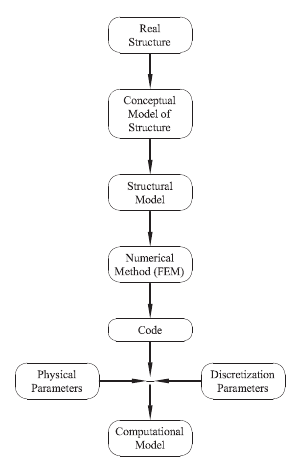
\includegraphics[width=0.5\textwidth,center]{Slike/Algoritam.png}
\caption{Алгоритам који приказује кораке потребне да би се дошло до применљивог кода од реалне конструкције \cite{eo1}}
\end{figure}
Данас је немогуће замислити брз и ефикасан прорачун конструкција без примене методе коначних елемената који се користе у софтверским пакетима. Технолошки напредак који су нам донели рачунари у грађевинарству су олакшали живот модерног инжењера али тај технолошки напредак који доноси доста аутоматизације је мач са две оштрице јер чине корисника лењим за критичким сагледавањем резултата. Овим семинарским радом ћемо показати колико места за грешку је могуће направити решавањем једноставних модела и зашто се на крају дана морамо ослањати на своје инжењерско знање стечено на факултету. 
\subsection{Задаци за израду семинарског рада}
Први задатак се састоји из прорачуна и приказивања матрице крутости коначног елемента типа Q9 применом неког од програмских језика (Matlab, Mathcad, Python итд).\\
Други задатак је прорачун деформације и напонског стања статичког система конзоле оптерећене концетрисаном силом на слободном крају коришћењем једног од претходно наведених програмских језика за срачунату матрицу крутости из првог задатка.\\
За трећи задатак је потребно коришћењем једног комерцијалног програма извући упоредне резултате варирањем димензија греде, стубова и растојања стубова континуалне греде оптерећене једнакоподељеним оптерећењем и дати закључак.
\newpage
\section{Први задатак}
\subsection{Теоријска позадина извођења матрице крутости}
Приказаћемо поступак добијања матрице крутости уз помоћ основних принципа механике.
\par
Основне једначине теорије еластичности могу да се опишу на два начина:
\begin{enumerate}
\item Математичком формулацијом које са граничним условима чине потпуно дефинисан проблем
\item Вариjационим формулама
\end{enumerate}
Математичким формулацијама са граничним условима можемо да решимо само једноставне проблеме, за комплексније проблеме нам стоји на располагању варијациона формулација у којој спада принцип виртуалног рада односно принцип виртуалних померања.\\
Виртуелна померања $\delta u$ \cite{mnd1} су произвољна, бесконачно мала померања (непрекидне, диференцијабилне функције координата тачака) која задовољавају граничне услове по померањима.\par
Нека је тело запремине $V$ ограничено површи \textit{Г} оптерећено запреминским $f$ и површинским $p$ оптерећењем са граничним условима које су на граничној површи (контури) дати по померањима \textit{Гu} и по силама \textit{Гs}.
\begin{figure}[H]
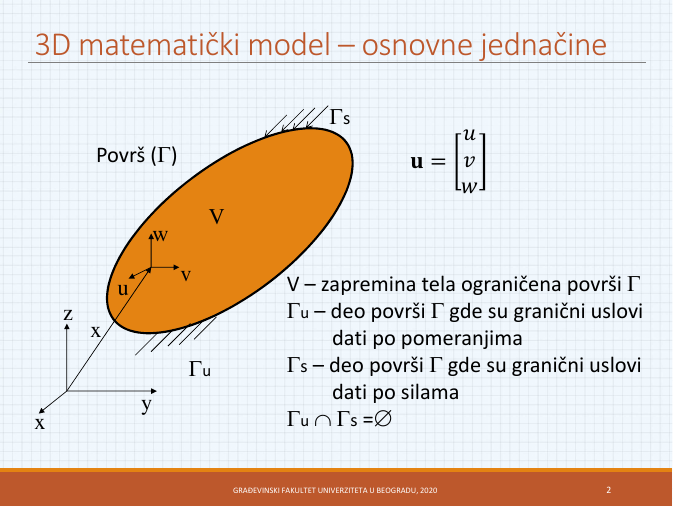
\includegraphics[width=0.9\textwidth, height=10cm]{Slike/Telo.png}
\caption{Тело ограничено површи Г \cite{mnd1}}
\end{figure}
Из тродимензионалог тела издвајамо елементарни део чија је запремина $dV$:
\begin{figure}[H]
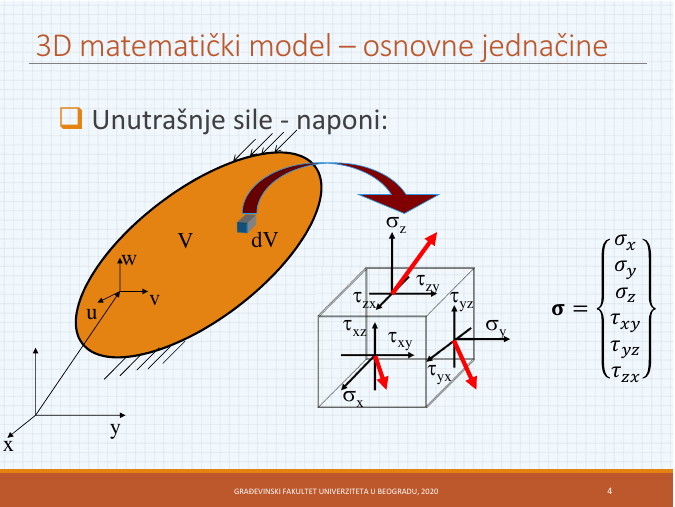
\includegraphics[width=0.9\textwidth, height=10cm]{Slike/TenzorNapona.png}
\caption{Тензор напона за елементарни део тела \cite{mnd1}}
\end{figure}
За систем кажемо да је у равнотежи ако је збир парцијалних извода напона $\mathbb{ \sigma }$  са вектором оптерећења $f$ за одређену раван једнак нули, тј:
\begin{eqnarray}
\mathbb{L}^T \cdot \mathbb{\sigma} + f = 0
\end{eqnarray}
Где су:
\begin{eqnarray*}
\mathbb{L}^T &=& 
\begin{bmatrix}
\frac{\partial}{\partial x} & 0 & 0\\
0 & \frac{\partial}{\partial y} & 0\\
0 & 0 & \frac{\partial}{\partial z}\\
\frac{\partial}{\partial y} & \frac{\partial}{\partial x} & 0\\
0 & \frac{\partial}{\partial z} & \frac{\partial}{\partial y}\\
\frac{\partial}{\partial z} & 0 & \frac{\partial}{\partial x}
\end{bmatrix}
\text{- матрица оператор, матрица парцијелних извода}\\
\mathbb{ \sigma} &=&
 \begin{bmatrix}
\sigma_x & \tau_{xy} & \tau_{xz}\\
\tau_{yx} & \sigma_{y} & \tau_{yz}\\
\tau_{zx} & \tau_{zy} & \sigma_{z}
\end{bmatrix}
\text{- тензор напона елементарног тела } dV\\
f &=& 
\begin{bmatrix}
fx\\
fy\\
fz
\end{bmatrix} 
\text{- вектор запреминског оптерећења}
\end{eqnarray*}
Када се једначина $(5)$ множи се са вектором виртуалних померања $\delta u$ и интеграли по читавој запремини тела $V$ добија се следеће:
\begin{eqnarray}
\int _{V} L^T  \sigma \delta u d V + \int_{V} f \delta u^T dV = 0 
\end{eqnarray}
За део контуре код којег су гранични услови дати по силама, услов равнотеже између спољашњих и унутрашњих сила дат је једначинама познатијим као Кошијеви површински услови \cite{otpornost}:

\begin{eqnarray}
\sigma_x \cdot n_x + \tau_{xy} \cdot n_y + \tau_{xz} \cdot n_z = p_x \\
\tau_{yx} \cdot n_x + \sigma_{y} \cdot n_y + \tau_{yz} \cdot n_z = p_y \\
\tau_{zx} \cdot n_x + \tau_{zy} \cdot n_y + \sigma_{z} \cdot n_z = p_z
\end{eqnarray}
Или матрично:
\begin{eqnarray}
\sigma n = p
\end{eqnarray}
Где су:
\begin{eqnarray*}
n &=& \begin{bmatrix}
n_x & 0 & 0 & n_y & 0 & n_z\\
0 & n_y & 0 & n_x & n_z & 0\\
0 & 0 & n_z & 0 & n_y & n_x
\end{bmatrix} 
\text{- матрица триг. функција углова нормале }n \\
p &=& \begin{bmatrix}
p_x\\
p_y\\
p_z
\end{bmatrix}
\text{- вектор површинских сила у правцима } x,y,z
\end{eqnarray*}
Слично као и са једначином $(5)$ и Кошијеви површински услови се множе са вектором виртуалних померања $\delta u^T$ и интеграле по контури где су гранични услови дати по силама \textit{Гs}:
\begin{align}
\int_{\text{Гs}} (\sigma n -p) \delta u^T dA = 0 \label{Equ:C}
\end{align}
Сабирањем $(5)$ са $(11)$ при чему су:
\begin{eqnarray}
L \delta u &=& \delta \epsilon \\
L^T(\sigma \delta u^T) = L^T \sigma \delta u^T + \sigma L \delta u &\Rightarrow&  L^T \sigma \delta u^T = L^T (\sigma \delta u^T) - \sigma \delta \epsilon^T \\
\int_V L^T (\sigma \delta u^T)dV &=& \int_{\text {Гs}} \sigma \delta u^T n dA
\end{eqnarray}
Добијамо израз:
\begin{align}
\int_V \sigma \delta \epsilon^T dV - \int_V f \delta u^T dV - \int_{\text{Гs}} p \delta u^T dA = 0 \label{Equ:A}
\end{align}
Израз $(15)$ представља принцип виртуaлног рада који гласи : 
\par
За тело у равнотежи важи да је збир радова спољашњих и унутрашњих сила при виртуелним померањима једнак нули \cite{mnd1}, тј:
\begin{align}
\delta W_{ext} + \delta W_{int} = 0
\end{align}
Где су:
\begin{eqnarray*}
\delta W_{ext} &=& - \int_V f \delta u^T dV - \int_{\text{Гs}} p \delta u^T dA \text{ - рад спољашњих сила}\\
\delta W_{int} &=& \int_V \sigma \delta \epsilon^T dV \text{ - рад унутрашњих сила}
\end{eqnarray*}
Из конститутивних једначина је позната веза:
\begin{eqnarray}
\sigma = E \epsilon
\end{eqnarray}
Па је након сређивања заменом $\delta u^T L^T = \delta \epsilon^T$ рад унутрашњих сила коначно једнак:
\begin{eqnarray}
\delta W_{int} = \int_V \delta u^T L^T E L u dV 
\end{eqnarray}
Поље померања $u$ се апроксимира интерполационим функцијама $N$:
\begin{eqnarray}
u = Nq
\end{eqnarray}
За виртуелно померање $\delta u$ следи:
\begin{eqnarray}
\delta u = N \delta q \Rightarrow \delta u^T=  \delta q^T N^T
\end{eqnarray}
Како је:
\begin{eqnarray}
\epsilon = Lu \Rightarrow ^{u = Nq} \epsilon = LNq = Bq
\end{eqnarray}
Коначно је израз за напон $\sigma$ једнак:
\begin{eqnarray}
\sigma = E \epsilon = E B q
\end{eqnarray}
Заменом претходних израза у једначини $(3)$ и дељењем једначине са $ \delta q^T$ добијамо:
\begin{eqnarray}
\left( \int_V B^T E B dV \right) q = \int_V N^T f dV + \int_{\text{Гs}} N^T p  dA
\end{eqnarray}
Како је $Kq = Q$ примећујемо да израз $\left( \int_V B^T E B dV \right) $ представља матрицу крутости $K$, тј:
\begin{eqnarray}
K = \int_V B^T E B dV
\end{eqnarray}
За равански коначни елемент $Q9$ са константном дебљином $t$ матрица крутости има следећи облик:
\begin{align}
K = t\int_A B^T E B dA 
\end{align}
\subsection{Изопараметарска формулација Q9 коначног елемента и матрица крутости}
Природни координатни систем $(\xi, \eta)$ за $Q9$ коначни елемент је приказан на следећој слици:
\begin{figure}[H]
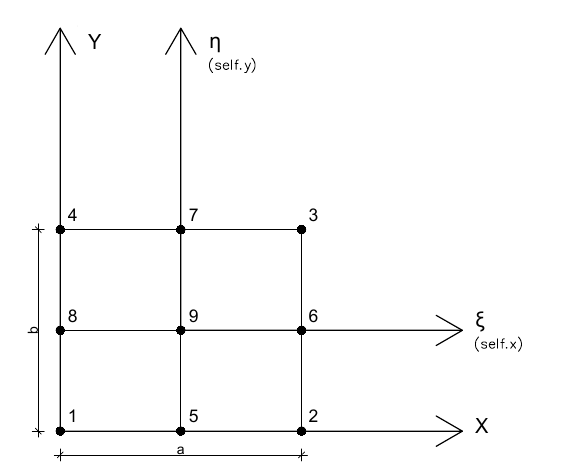
\includegraphics[width=\textwidth, height=10cm]{Slike/Q9_izoparametarski.png}
\caption{Природни координатни систем Q9 коначног елемента}
\end{figure}
Идеја увођења оваквог система је лакша интеграција произвољног правоугаоног коначног елемента са 9 тачака пошто су границе интеграције дефинисане од $[-1,1]$ у оба ортогонална правца за природни кооринатни систем. Приликом интеграције се природни координатни систем трансформише у глобални уз помоћ Јакобијеве матрице.\\
Координате тачака $i$ су дате у глобалном координатном систему $X,Y$ дефинисаном на слици 5 (тачка 1 нпр има координате $(0,0)$, тачка 2 (a, 0), итд) док су интерполационе функције $N_i(\xi, \eta)$ дефинисане у природном координатном систему.\\
Поља померања $u(\xi, \eta)$ и $v(\xi, \eta)$ су дефинисана на следећи начин:
\begin{eqnarray}
u(\xi, \eta) &=& \sum_{i=1} ^9 N_{i}(\xi, \eta)x_i\\
v(\xi, \eta) &=& \sum_{i=1} ^9 N_{i}(\xi, \eta)y_i
\end{eqnarray}
Где су $x_i$ и $y_i$ померања тачке $i$ у $X$ односно $Y$ правцу и оне чине основне непознате коначног елемента, интерполационе функције $N_i$ су дефинисане на следећи начин:
\begin{eqnarray}
N_1 &=& 0.25(1 - \xi)(1- \eta) - 0.5N_5 -0.5 N_8 - 0.25N_9\\
N_2 &=& 0.25(1 + \xi)(1-\eta) -0.5N_5 -0.5N_6 - 0.25N_9\\ 
N_3 &=& 0.25(1+ \xi)(1+\eta) -0.5N_6 -0.5N_7 -0.25N_9\\
N_4 &=&  0.25(1-\xi)(1+\eta) -0.5N_7 - 0.5N_8 - 0.25N_9\\
N_5 &=& 0.5(1 - \xi ^2)(1- \eta) -0.5N_9\\
N_6 &=& 0.5 (1+ \xi) (1- \eta ^ 2) -0.5 N_9\\
N_7 &=& 0.5(1 - \xi ^2)(1+ \eta) -0.5 N_9\\
N_8 &=& 0.5(1- \xi)(1-\eta ^2) -0.5N_9\\
N_9 &=& (1-\xi ^2)(1- \eta ^2)
\end{eqnarray}
Поље деформацијa је дефинисано у глобалном координатном систему оса као:
\begin{align}
\epsilon = 
\begin{bmatrix}
\epsilon_x \\
\epsilon_y \\
\gamma _{xy}
\end{bmatrix}
=
\begin{bmatrix}
\frac{\partial u}{\partial x}\\
\frac{\partial v}{\partial y}\\
\frac{\partial u}{\partial y} + \frac{\partial v}{\partial x}
\end{bmatrix}
\end{align}
Како су поља померања $u$ и $v$ у дефинисана у изопараметарском координатном систему $(\xi, \eta)$ а поља деформација у глобалном, тј поља померања из којих следе поља деформација у координатном систему $(X,Y)$ потребно је пронаћи одговарајућу везу између њих,
то радимо на следећи начин:
\begin{eqnarray}
\frac{\partial u}{\partial x} &=& \frac{\partial u}{\partial \xi} \cdot \frac{\partial \xi}{\partial x} + \frac{\partial u}{\partial \eta} \cdot \frac{\partial \eta}{\partial y}
\end{eqnarray}
Издвајањем $\frac{\partial u}{\partial \xi}$ и $\frac{\partial u}{\partial \eta}$ се добија:
\begin{eqnarray}
\frac{\partial u}{\partial \xi} &=& \frac{\partial u}{\partial x} \cdot \frac{\partial x}{\partial \xi} + \frac{ \partial u}{\partial y} \cdot \frac{\partial y}{\partial \xi}\\
\frac{\partial u}{\partial \eta} &=& \frac{\partial u}{\partial x} \cdot \frac{\partial x}{\partial \eta} + \frac{\partial u}{\partial y} \cdot \frac{\partial y}{\partial \eta}
\end{eqnarray}
Или матрично:
\begin{eqnarray}
\begin{bmatrix}
\frac{\partial u}{\partial \xi}\\
\frac{\partial u}{\partial \eta}
\end{bmatrix}
=
\begin{bmatrix}
\frac{\partial x}{\partial \xi} & \frac{\partial y}{\partial \xi} \\
\frac{\partial x}{\partial \eta} & \frac{\partial y}{\partial \eta}
\end{bmatrix}
\cdot
\begin{bmatrix}
\frac{\partial u}{\partial x} \\
\frac{ \partial u}{\partial y}
\end{bmatrix}
\end{eqnarray}
Где је:
\begin{eqnarray}
\mathbb{J} = 
\begin{bmatrix}
\frac{\partial x}{\partial \xi} & \frac{\partial y}{\partial \xi} \\
\frac{\partial x}{\partial \eta} & \frac{\partial y}{\partial \eta}
\end{bmatrix}
\text{- Јакобијева матрица}
\end{eqnarray}
Елементи Јакобијеве матрице су у ствари одговарајући парцијални изводи поља померања $x$ и $y$ где су:
\begin{eqnarray}
\frac{\partial x}{\partial \xi} &=& \sum_{i=1} ^ 9 \frac{\partial N_i(\xi, \eta)}{\partial \xi} \cdot x_i \quad \frac{\partial y}{\partial \xi} = \sum_{i=1} ^ 9 \frac{\partial N_i(\xi, \eta)}{\partial \xi} \cdot y_i \\
\frac{\partial x}{\partial \eta} &=& \sum_{i=1} ^ 9 \frac{\partial N_i(\xi, \eta)}{\partial \eta} \cdot x_i \quad \frac{\partial y}{\partial \eta} = \sum_{i=1} ^ 9 \frac{N_i(\xi, \eta)}{\partial \eta} \cdot y_i
\end{eqnarray}
Па се Јакобијева матрица може приказати и као:
\begin{eqnarray}
\mathbb{J} = 
\begin{bmatrix}
\sum_{i=1} ^ 9 \frac{\partial N_i(\xi, \eta)}{\partial \xi} \cdot x_i & \sum_{i=1} ^ 9 \frac{\partial N_i(\xi, \eta)}{\partial \xi} \cdot y_i \\
\sum_{i=1} ^ 9 \frac{\partial N_i(\xi, \eta)}{\partial \eta} \cdot x_i & \sum_{i=1} ^ 9 \frac{\partial N_i(\xi, \eta)}{\partial \eta} \cdot y_i
\end{bmatrix}
\end{eqnarray}
Како су поља деформација $\varepsilon$ (37) дефинисана као одговарајући парцијелни изводи поља померања  по $x$ и $y$ а поља померања су функције интерполационих функција у глобалном координатном систему потребно је успоставити везу између интерполационих функција у глобалном координатном систему $(X,Y)$ и интерполационих функција у природном координатом систему $(\xi, \eta)$. Везу између два координатна система, тј интерполационих функција у два различита координатна система успоставља претходно изведена Јакобијева матрица $\mathbb{J}$:
\begin{eqnarray}
\begin{Bmatrix}
\frac{ \partial N_i}{\partial x}\\
\frac{\partial N_i}{\partial y}
\end{Bmatrix}
= \mathbb{J} ^ {-1} 
\begin{Bmatrix}
\frac{ \partial N_i}{\partial \xi}\\
\frac{\partial N_i}{\partial \eta}
\end{Bmatrix}
\end{eqnarray}
Са претходном везом можемо да формирамо матрицу $\mathbb{B}$:
\begin{eqnarray}
\mathbb{B}(x,y) = 
\begin{bmatrix}
\frac{\partial N_1}{\partial x} & 0 & \frac{\partial N_2}{\partial x} & 0 & 
 \hdots & \frac{\partial N_9}{\partial x} & 0 \\
0 & \frac{\partial N_1}{\partial y} & 0 & \frac{\partial N_2}{\partial y} & \hdots & 0 &  \frac{\partial N_9}{\partial y} \\
\frac{\partial N_1}{\partial y} & \frac{\partial N_1}{\partial x} & \frac{\partial N_2}{\partial y} &
\frac{\partial N_2}{\partial x}   & \hdots &
\frac{\partial N_9}{\partial y} & \frac{\partial N_9}{\partial y}    
\end{bmatrix}
\end{eqnarray}
Коначно матрица крутости (25) се може представити на следећи начин:
\begin{eqnarray}
K = t\int_{-1} ^1  \int_{-1} ^1 B(x,y)^T E B(x,y) |J| d \xi d \eta
\end{eqnarray}
\subsection{Примена Python програмског језика за формирање матрице крутости Q9 коначног елемента}
Приликом писања скрипти је коришћен објектно оријентисани приступ искључиво из разлога изолације променљивих унутар метода пошто Python уме да "заборави" променљиве приликом њихове алокације у меморији.\\
За симболичку интеграцију се користи библиотека \textit{sympy} \cite{sympy} уз стандардне библиотеке које нуди $Python3$ програмски језик.
Приликом прорачуна матрице крутости матрица материјала $\mathbb{E}$ је дата за равно стање напона:
\begin{eqnarray}
\mathbb{E} = \frac{E}{1 - \nu^2}
\begin{bmatrix}
 1 & \nu & 0\\
 \nu & 1 & 0\\
 0 & 0 & \frac{1 - \nu}{2}
\end{bmatrix}
\end{eqnarray}
 Kоја је у коду представљена у \textit{init} методи:
\begin{lstlisting}

self.Ematrica = sp.Matrix([[self.E/(1-self.ni**2), self.ni*self.E/(1-self.ni**2), 0],
                                   [self.ni*self.E/(1-self.ni**2), self.E/(1-self.ni**2), 0],
                                   [0, 0, (1-self.ni)/2*self.E/(1-self.ni**2)]
                                   ])
                                   
\end{lstlisting}

Низови координата тачака \texttt{x\_niz} и \texttt{y\_niz} у глобалном координатом систему $(X,Y)$ коначног елемента какав је приказан на слици 5 су дати у помоћној скрипти $mapiranjeQ9.py$ као методе:

\begin{lstlisting}
    def x_niz(self): # Formiranje koordinata tacaka Xi
        niz = sp.Matrix([0, self.a, self.a, 0, 0.5 * self.a, self.a, 0.5 * self.a, 0, 0.5 * self.a])
        return niz

    def y_niz(self): # Formiranje koordinata tacaka Yi
        niz = sp.Matrix([0, 0, self.b, self.b, 0, 0.5 * self.b, self.b, 0.5 * self.b, 0.5 * self.b])
        return niz
\end{lstlisting}

Јакобијева матрица, њена инверзна и детерминанта су приказане у следећим методама у скрипти $mapiranjeQ9.py$:

\begin{lstlisting}
        def Jakobijan(self):
        niz_interpolacionih = sp.Matrix([self.N1(), self.N2(), self.N3(), self.N4(), self.N5(), self.N6(), self.N7(), self.N8(), self.N9()])
        x_niz = self.x_niz()
        X = sp.transpose(x_niz)*niz_interpolacionih # Polje pomeranja u X pravcu
        X = X[0]
        y_niz = self.y_niz()
        Y = sp.transpose(y_niz)*niz_interpolacionih # Polje pomeranja u Y pravcu
        Y = Y[0]
        J = sp.Matrix([[sp.diff(X, self.x), sp.diff(Y, self.x)], [sp.diff(X, self.y), sp.diff(Y, self.y)]])
        return J
    
    def JakobijanInv(self):
        J = self.Jakobijan()
        J = J.inv()
        return J

    def JakobijanDet(self):
        J = self.Jakobijan()
        J = J.det()
        return J
\end{lstlisting}

Формирање матрице $\mathbb{B}$ спајањем матрица $\mathbb{B}_i$ по колонама је представљено у методи:
\begin{lstlisting}
# Formiranje matrice B spajanjem matrica Bi:
   def Bmatrica(self):
        b = self.mp.B1().col_insert(2, self.mp.B2())
        b = b.col_insert(4, self.mp.B3())
        b = b.col_insert(6, self.mp.B4())
        b = b.col_insert(8, self.mp.B5())
        b = b.col_insert(10, self.mp.B6())
        b = b.col_insert(12, self.mp.B7())
        b = b.col_insert(14, self.mp.B8())
        b = b.col_insert(16, self.mp.B9())
        return b
\end{lstlisting}
Где су матрице $\mathbb{B}_i$ матрице из скрипте $mapiranjeQ9.py$. Пример дела кода из скрипте $mapiranjeQ9.py$ којом је представљена матрица $\mathbb{B}_1$:

\begin{lstlisting}
#Kolone matrice B pri cemu su kolone matrice reda 3x2
def B1(self):
        vektor = self.JakobijanInv()*sp.Matrix([[sp.diff(self.N1(), self.x)], [sp.diff(self.N1(), self.y)]])
        x = vektor[0]
        y = vektor[1]
        matrica = sp.Matrix([[x, 0], [0, y], [y, x]])
        return matrica
\end{lstlisting}

Подинтегрална функција и њена интеграција са могућношћу исписивања елемента матрице крутости у симболичкој или интегралној форми као и исписивање целе матрице крутости је приказано у следећој методи:
\begin{lstlisting}
# Formiranje podintegralne f-je i integracija:
    def integracija(self):
        BT = self.BT()
        B = self.Bmatrica()
        upit = str(input('Numericka ili simbolicka vrednost koeficijenta krutosti matrice? (recima unesi "numericka" ili "simbolicka", bez navodnika): '))
        upit = upit.lower()
        if upit == 'simbolicka':
            i = input('Unesi red matrice i: ')
            j = input('Unesi kolonu matrice j: ')
            if i == 'sve' and j == 'sve':
                podintegralna = BT*self.Ematrica*B*self.t*self.mp.JakobijanDet()
                integral = sp.integrate(sp.integrate(podintegralna, (self.x, -1, 1)), (self.y, -1, 1))
                print('\nK = ', integral)
            else:
                i = int(i)
                j = int(j)
                if i > 18 and j > 18:
                    print('\ni i j moraju biti manji od 18! ')
                    exit()
                else:
                    podintegralna = BT.row(i - 1)*self.Ematrica*B.col(j - 1)*self.t*self.mp.JakobijanDet()
                    integral = sp.integrate(sp.integrate(podintegralna, (self.x, -1, 1)), (self.y, -1, 1))
                    koeficijent_matrice = integral[0]
                    print(f'\nk{i}_{j} =', koeficijent_matrice)
        elif upit == 'numericka':
            i = input('Unesi red matrice i: ')
            j = input('Unesi kolonu matrice j: ')
            if i == 'sve' and j == 'sve':
                a = float(input('Unesi dimenziju konacnog elementa a [m]: '))
                b = float(input('Unesi dimenziju konacnog elementa b [m]: '))
                E = float(input('Unesi moduo elasticnosti E [GPa]: '))
                E = E * 10 ** 6
                ni = float(input('Unesi Poasonov koeficijent \u03BD: '))
                t = float(input('Unesi debljinu konacnog elementa t [m]: '))
                podintegralna = BT*self.Ematrica*B*self.t*self.mp.JakobijanDet()
                integral = sp.integrate(sp.integrate(podintegralna, (self.x, -1, 1)), (self.y, -1, 1))
                integral = integral.subs({self.E: E, self.ni: ni, self.t: t, self.a: a, self.b: b})
                print('\nK = ', integral)

            elif i != 'sve' and j != 'sve':
                i = int(i)
                j = int(j)
                if i > 18 or j > 18:
                    print('\ni i j moraju biti manji od 18! ')
                    exit()
                else:
                    a = float(input('Unesi dimenziju konacnog elementa a [m]: '))
                    b = float(input('Unesi dimenziju konacnog elementa b [m]: '))
                    E = float(input('Unesi moduo elasticnosti E [GPa]: '))
                    E = E*10**6
                    ni = float(input('Unesi Poasonov koeficijent \u03BD: '))
                    t = float(input('Unesi debljinu konacnog elementa t [m]: '))
                    podintegralna = BT.row(i - 1) * self.Ematrica * B.col(j - 1) * self.t*self.mp.JakobijanDet()
                    integral = sp.integrate(sp.integrate(podintegralna, (self.x, -1, 1)), (self.y, -1, 1))
                    integral = integral.subs({self.E: E, self.ni: ni, self.t: t, self.a: a, self.b: b})
                    koeficijent_matrice = integral[0]
                    print(f'\nk{i}_{j} =', koeficijent_matrice)
            else:
                print('\n i i j moraju biti rec "sve" ili broj manje ili jednak 18!')
                exit()
        else:
            print('\nUnesi lepo "simbolicka" ili "numericka" pri upitu.')
            exit()

\end{lstlisting}
Приликом читања кода имати у виду да се променљиве \texttt{self.x} и \texttt{self.y} односе на променљиве изопараметарског координатог система тј \texttt{self.x} = $\xi$ и \texttt{self.y} = $\eta$.\\ Приликом уношења "sve" за упите променљивих \texttt{i} и \texttt{j} имати у виду да ће приказ резултата потрајати у зависности од радног такта процесора рачунара.
\newpage
\section{Други задатак}
\subsection{Алгоритам прорачуна напона и деформација конзолног носача оптерећеног концентрисаном силом на слободном крају методом коначних елемената}
Алгоритам коришћен за прорачун конзолног носача је следећи:
\begin{enumerate}
\item Поделити носач на коначне елементе водећи рачуна о њиховој регуларности. 
\item Нумерисати померања $q$ у чворовима у оба правца и формирати кодиран вектор померања.
\item Заменити позната померања $q_p$ њиховим вредностима.
\item Формирати вектор концентрисаних сила кодиран као и вектор померања и задати вредност концентрисане силе у правцу одређеног померања.
\item Формирати кодирану матрицу крутости за цео систем.
\item Одредити непозната померања.
\item Одредити деформације у чворовима коначних елемената.
\item Одредити напоне у чворовима коначних елемената и упросечити их ако је чвор заједнички за више коначних елемената.
\item Приказати резултате.
\end{enumerate}
Прорачун је спроведен за две различите густине мреже коначних елемената: ређом са укупно 4 коначних елемената и са односом страна $\frac{b}{a}= \frac{1}{1.25} = 0.8$ и гушћом са укупно 16 коначних елемената и са односом страна $\frac{b}{a}= \frac{0.5}{0.625} = 0.8$. Како је однос страна исти вредности елемената матрице крутости за један коначни елемент се неће променити за ове две различите густине. Усвојена конвенција померања и коначних елемената за различите густине су приказане на следећим сликама:
\begin{figure}[H]
\centering
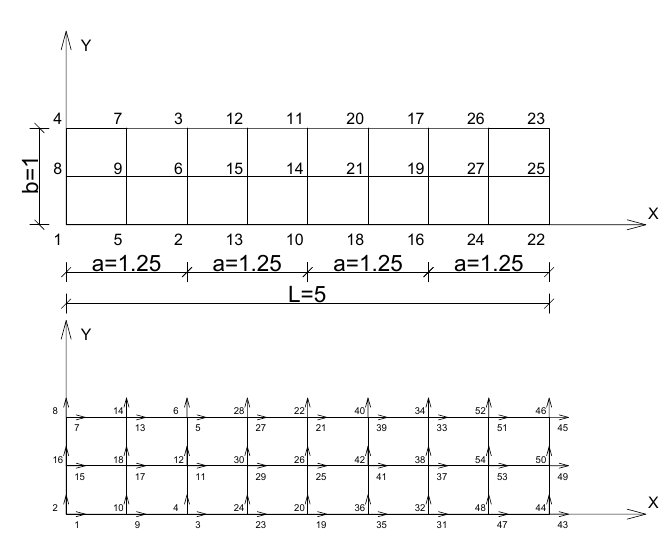
\includegraphics[width=10cm, height=5cm]{Slike/Redja.png}
\caption{Нумерација чворова конзолног носача са мрежом од 4 коначна елемента (слика горе), нумерација (кодни бројеви) померања у чворовима конзолног носача са мрежом од 4 коначна елемента (слика доле)}
\end{figure}
\begin{figure}[H]
\centering
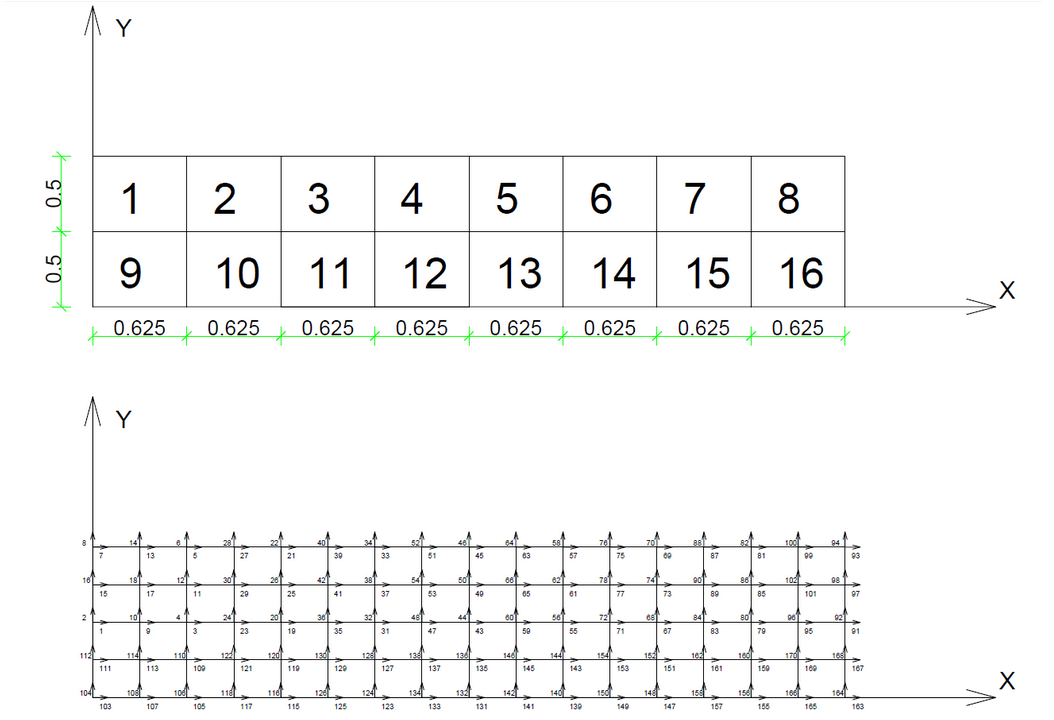
\includegraphics[width=10cm, height=7cm]{Slike/Gusca.png}
\caption{Нумерација коначних елемената конзолног носача са мрежом од 16 коначних елемената (слика горе), нумерација (кодни бројеви) померања конзолног носача са мрежом од 16 коначних елемената (слика доле)}
\end{figure}
Скрипта као резултат враћа дијаграме померања и напона за различите густине коначног елемента и то за горње влакно носача, напони су упросечени у тачакма поклапања коначних елемената. \\
Приликом покретања скрипте за жељену густину откоментарисати \texttt{obj.plot()} или \texttt{obj.plot2x()} брисањем карактера $\#$.
\subsection{Примена Python програмског језика за решавање конзолног носача}
Додатне библиотеке за операције са низовима, матрицама и њихово кодирање омогућавају \texttt{numpy} \cite{numpy} и \texttt{pandas} \cite{pandas}, библиотека за штампање дијаграма омогућава \texttt{matplotlib} \cite{matplotlib}. \\
Како постоје посебне методе за различите густине мреже коначних елемената биће приказане само методе и њихово функционисање за мрежу са 4 коначна елемента, аналогно важи код и за гушћу мрежу само са разликом у броју померања.
\par
Првенствено у \texttt{init(self)} методи се складишти као атрибут  \\
\texttt{self.niz\_elemenata} низ вредности елемената матрице крутости читајући колону "Elementi" из $ElementiMK.csv$ фајла.\\
Методом \texttt{index(self)} се врши кодирање померања коначних елемената где су врсте посебно померања чворова једног коначног елемента, метода враћа само матрицу кодова (индекса) померања коначних елемената:
\begin{lstlisting}
    def index(self):
        matrica = np.array([
            [1, 2, 3, 4, 5, 6, 7, 8, 9, 10, 11, 12, 13, 14, 15, 16, 17, 18],  # KE 1
            [3, 4, 19, 20, 21, 22, 5, 6, 23, 24, 25, 26, 27, 28, 11, 12, 29, 30],  # KE 2
            [19, 20, 31, 32, 33, 34, 21, 22, 35, 36, 37, 38, 39, 40, 25, 26, 41, 42],  # KE 3
            [31, 32, 43, 44, 45, 46, 33, 34, 47, 48, 49, 50, 51, 52, 37, 38, 53, 54]  # KE 4
            ])
        return matrica
\end{lstlisting}
Метода \texttt{indeksiranematrice(self)} формира матрицу крутости 18x18 трансформишући претходно учитани низ елемената матрица крутости и коначно враћа низ 4 кодираних матрица крутости (4x18x18) кодиране како и у \texttt{index(self)} методи:

\begin{lstlisting}
def indeksiranematrice(self):
        matrica_krutosti = self.niz_elemenata.reshape(18, 18)
        indeks_matrica = pd.DataFrame(self.index())  
        konacni_elementi = np.arange(0, 4)  
        niz_matrica = []
        for i in konacni_elementi:
            indeks_matrice_i = np.array(indeks_matrica.loc[i])
            matrica = pd.DataFrame(matrica_krutosti, index=indeks_matrice_i, columns=indeks_matrice_i)
            niz_matrica.append(matrica)
        return niz_matrica
\end{lstlisting}
Када имамо низ кодираних матрица крутости можемо да формирамо матрицу крутости $\mathbb{K}$ целог система:
\begin{lstlisting}
def ksystem(self):
        pomeranja = np.array(np.arange(1, 55))  
        ksistema = pd.DataFrame(np.zeros((54, 54)), columns=pomeranja, index=pomeranja) 
        matrice_krutosti = self.indeksiranematrice()
        for m in matrice_krutosti:
            for i in ksistema.index:
                for j in ksistema.columns:
                    try:
                        ksistema.loc[i][j] = ksistema.loc[i][j] + m.loc[i][j]
                    except Exception:
                        pass
        return ksistema
\end{lstlisting}

Са формираном матрицом крутости целог система потребно је формирати матрицу крутости уз непозната померања  $\mathbb{K}_{nn}$  избацивањем редова и колона са индексима (познатим померањима) $(1, 2, 15, 16, 7, 8)$  и на исти начин формирати вектор чворних сила $P_{n}$. Вектор чворних сила $P_{n}$ за све своје елементе има вредност $0$ осим за елемент са индексом (кодом померања) $50$ чија је вредност једнака $-40kN$ по поставци задатка. Резултат методе \texttt{unknown\_displacements(self)} је вектор непознатих померања $q_{n}$ који се добија познатом везом:

\begin{eqnarray}
q_{n} = \mathbb{K}_{nn} ^ {-1} P_{n}
\end{eqnarray} 
Метода \texttt{unknown\_displacements(self)}:
\begin{lstlisting}
def unknown_displacements(self):
        vektor_cvornih_sila = np.array(np.zeros(54), dtype=np.int64)  
        pomeranja = np.array(np.arange(1, 55))  
        cvorne_sile = pd.Series(vektor_cvornih_sila, index=pomeranja)
        for i in cvorne_sile.index:
            if i == 50:  # i za 4 KE je 50
                cvorne_sile.loc[50] = cvorne_sile.loc[50] - 40
        poznata_pomeranja = np.array([1, 2, 15, 16, 7, 8])  
        nepoznata_pomeranja = pd.Series(pomeranja, index=pomeranja).drop(poznata_pomeranja)
        pnn = cvorne_sile.drop(poznata_pomeranja)
        knn = self.ksystem().drop(index=poznata_pomeranja, columns=poznata_pomeranja)
        qnn = np.dot(np.linalg.inv(knn), pnn)
        qnn = pd.Series(qnn, index=nepoznata_pomeranja)
        return qnn
\end{lstlisting}
Када смо одредили непозната померања можемо да формирамо вектор свих померања чворова $q$, метода \texttt{displacements(self)} враћа кодирани вектор померања свих чворова система:
\begin{lstlisting}
   def displacements(self):
       qnn = self.unknown_displacements2x()
       q = pd.Series(np.zeros(54), index=np.arange(1, 55))  
       for i in q.index:
           try:
               q.loc[i] = q.loc[i] + qnn.loc[i]
           except Exception:
               pass
       return q
\end{lstlisting}
Са формираним вектором померања чворова постоји све што је потребно да се одреде деформације а потом и напони у чворовима коначних елемената. Како су поља деформација $\varepsilon$ (37) одређени парцијелни изводи поља померања $u(x,y)$ и $v(x,y)$ а поља померања су дефинисана у природном координатном систему $(\xi, \eta)$ тј:
\begin{eqnarray*}
u(\xi, \eta) &=& N_1 q_{x1} + N_2q_{x2} + N_3q_{x3} + N_4q_{x4} + N_5q_{x5} + N_6q_{x6} + N_7q_{x7} + N_8q_{x8} + N_9q_{x9} \\
v(\xi, \eta) &=& N_1 q_{y1} + N_2q_{y2} + N_3q_{y3} + N_4q_{y4} + N_5q_{y5} + N_6q_{y6} + N_7q_{y7} + N_8q_{y8} + N_9q_{y9}\\
N_i &-& \text{ интерполациона функција i}\\
q_{xi} &-& \text{ померање i у X правцу}\\
q_{yi} &-& \text{ померање i у Y правцу}
\end{eqnarray*} 
Потребно је дефинисати изразе за поља померања у природном координатном систему. Без посебног извођења она су дефинисана као:
\begin{eqnarray}
\varepsilon(\xi, \eta) &=& t M 
\begin{bmatrix}
\frac{\partial u}{\partial \xi}\\
\frac{\partial u}{\partial \eta}\\
\frac{\partial v}{\partial \xi}\\
\frac{\partial v}{\partial \eta}
\end{bmatrix}
\end{eqnarray}
Где су:
\begin{eqnarray}
t &=& 
\begin{bmatrix}
1 & 0 & 0 & 0 \\
0 & 0 & 0 & 1\\
0 & 1 & 1 & 0
\end{bmatrix}
\\
M &=& 
\begin{bmatrix}
	\begin{bmatrix}
	\mathbb{J}^{-1}
	\end{bmatrix}
	&
	\begin{bmatrix}
	0 & 0 \\
	0 & 0
	\end{bmatrix}
	\\
	\begin{bmatrix}
	0 & 0 \\
	0 & 0
	\end{bmatrix}
	&
	\begin{bmatrix}
	\mathbb{J}^{-1}
	\end{bmatrix}
\end{bmatrix} \\
\mathbb{J} &=& 
\begin{bmatrix}
\frac{\partial x}{\partial \xi} & \frac{\partial y}{\partial \xi} \\
\frac{\partial x}{\partial \eta} & \frac{\partial y}{\partial \eta}
\end{bmatrix} \text{ - Јакобијева матрица}
\end{eqnarray}
Симболички прорачун деформацијиских величина у тачкама од 1-9 како су приказане на слици 5 посебно за сваку тачку раде методе \texttt{epsiloni} из скрипте $mapiranjeQ9.py$, методе враћају низ (вектор) од 3 елемента деформацијиских величина у симболичкој форми. Пример једне такве методе за тачку 1 коначног елемента:
\begin{lstlisting}
def epsilon1(self):
        Jakobijan = sp.Matrix([[sp.diff(self.polje_pomeranja_x(), self.x)], [sp.diff(self.polje_pomeranja_x(), self.y)], [sp.diff(self.polje_pomeranja_y(), self.x)], [sp.diff(self.polje_pomeranja_y(), self.y)]])
        inv_J = self.JakobijanInv()
        M = sp.Matrix([[inv_J[0], inv_J[1], 0, 0], [inv_J[2], inv_J[3], 0, 0], [0, 0, inv_J[0], inv_J[1]], [0, 0, inv_J[2], inv_J[3]]])
        t_matrica = sp.Matrix([[1, 0, 0, 0], [0, 0, 0, 1], [0, 1, 1, 0]])
        epsilon = t_matrica*M*Jakobijan
        epsilon = epsilon.subs({self.x: -1, self.y: -1})
        epsilon = np.array([epsilon[0], epsilon[1], epsilon[2]], dtype=str)
        return epsilon
\end{lstlisting}
Са изразима за деформацијиске величине можемо одредити напоне у тачкама коначних елемената уз помоћ Хуковог закона:
\begin{eqnarray}
\sigma = E \epsilon
\end{eqnarray}
У коду тај прорачун врши метода \texttt{stress(self, ke, tacka, q, napon)} која за дате параметре враћа низ (вектор) напона:
\begin{eqnarray}
\sigma = 
\begin{Bmatrix}
\sigma_x \\
\sigma_y \\
\tau_{xy}
\end{Bmatrix}
\end{eqnarray}
Параметар \texttt{ke} представља број коначног елемента (за 4 КЕ тај број је 1-4), параметар \texttt{tacka} је у ствари деформацијиско стање у тачки коначног елемента какве су приказане на слици 5 коју враћају методе \texttt{epsiloni}, параметар \texttt{q} је вектор померања система, и параметар \texttt{napon} има вредности: 0 - за приказ напона $\sigma_x, 1$ - за приказ напна $\sigma_y$ и 2 - за приказ напона $\tau_{xy}$:
\begin{lstlisting}
    def stress(self, ke, tacka, q, napon):
        indeksi = self.index()
        Q = [q[j] for j in indeksi[ke - 1]]
        X = [Q[2 * j] for j in range(9)]
        Y = [Q[2 * j + 1] for j in range(9)]
        a = self.a
        b = self.b
        qx1 = X[0]
        qx2 = X[1]
        qx3 = X[2]
        qx4 = X[3]
        qx5 = X[4]
        qx6 = X[5]
        qx7 = X[6]
        qx8 = X[7]
        qx9 = X[8]
        qy1 = Y[0]
        qy2 = Y[1]
        qy3 = Y[2]
        qy4 = Y[3]
        qy5 = Y[4]
        qy6 = Y[5]
        qy7 = Y[6]
        qy8 = Y[7]
        qy9 = Y[8]
        epsilon1 = eval(tacka[0])
        epsilon2 = eval(tacka[1])
        epsilon3 = eval(tacka[2])
        konacno = np.dot(self.E_matrica(), np.array([[epsilon1], [epsilon2], [epsilon3]]))
        konacno = konacno[napon][0]
        return konacno
\end{lstlisting}
Штампање дијаграма врши метода \texttt{plot(self)} формирајући низове вредности у тачкама горњег влакна:
\begin{lstlisting}
    def plot(self):
        q = self.displacements()
        kt = mp.KoordinateTacaka()
        q = pd.Series(q, index=np.arange(1, 55))
        ugib = [q.loc[16], q.loc[18], q.loc[12], q.loc[30], q.loc[26], q.loc[42], q.loc[38], q.loc[54], q.loc[50]]
        sigma_x = np.array([self.stress(ke=1, tacka=kt.epsilon4(), q=q, napon=0),
                            self.stress(ke=1, tacka=kt.epsilon7(), q=q, napon=0),
                            self.average(a=self.stress(ke=1, tacka=kt.epsilon3(), q=q, napon=0),
                                         b=self.stress(ke=2, tacka=kt.epsilon4(), q=q, napon=0)),
                            self.stress(ke=2, tacka=kt.epsilon7(), q=q, napon=0),
                            self.average(a=self.stress(ke=2, tacka=kt.epsilon3(), q=q, napon=0),
                                         b=self.stress(ke=3, tacka=kt.epsilon4(), q=q, napon=0)),
                            self.stress(ke=3, tacka=kt.epsilon7(), q=q, napon=0),
                            self.average(a=self.stress(ke=3, tacka=kt.epsilon3(), q=q, napon=0),
                                         b=self.stress(ke=4, tacka=kt.epsilon4(), q=q, napon=0)),
                            self.stress(ke=4, tacka=kt.epsilon7(), q=q, napon=0),
                            self.stress(ke=4, tacka=kt.epsilon3(), q=q, napon=0)
                            ])
        sigma_y = np.array([self.stress(ke=1, tacka=kt.epsilon4(), q=q, napon=1),
                            self.stress(ke=1, tacka=kt.epsilon7(), q=q, napon=1),
                            self.average(a=self.stress(ke=1, tacka=kt.epsilon3(), q=q, napon=1),
                                         b=self.stress(ke=2, tacka=kt.epsilon4(), q=q, napon=1)),
                            self.stress(ke=2, tacka=kt.epsilon7(), q=q, napon=1),
                            self.average(a=self.stress(ke=2, tacka=kt.epsilon3(), q=q, napon=1),
                                         b=self.stress(ke=3, tacka=kt.epsilon4(), q=q, napon=1)),
                            self.stress(ke=3, tacka=kt.epsilon7(), q=q, napon=1),
                            self.average(a=self.stress(ke=3, tacka=kt.epsilon3(), q=q, napon=1),
                                         b=self.stress(ke=4, tacka=kt.epsilon4(), q=q, napon=1)),
                            self.stress(ke=4, tacka=kt.epsilon7(), q=q, napon=1),
                            self.stress(ke=4, tacka=kt.epsilon3(), q=q, napon=1)
                            ])
        tau_xy = np.array([self.stress(ke=1, tacka=kt.epsilon4(), q=q, napon=2),
                           self.stress(ke=1, tacka=kt.epsilon7(), q=q, napon=2),
                           self.average(a=self.stress(ke=1, tacka=kt.epsilon3(), q=q, napon=2),
                                        b=self.stress(ke=2, tacka=kt.epsilon4(), q=q, napon=2)),
                           self.stress(ke=2, tacka=kt.epsilon7(), q=q, napon=2),
                           self.average(a=self.stress(ke=2, tacka=kt.epsilon3(), q=q, napon=2),
                                        b=self.stress(ke=3, tacka=kt.epsilon4(), q=q, napon=2)),
                           self.stress(ke=3, tacka=kt.epsilon7(), q=q, napon=2),
                           self.average(a=self.stress(ke=3, tacka=kt.epsilon3(), q=q, napon=2),
                                        b=self.stress(ke=4, tacka=kt.epsilon4(), q=q, napon=2)),
                           self.stress(ke=4, tacka=kt.epsilon7(), q=q, napon=2),
                           self.stress(ke=4, tacka=kt.epsilon3(), q=q, napon=2)
                           ])
        x_osa = np.linspace(0, 5, num=9)  # 4 KE
        fig, axs = plt.subplots(2, 2)
        axs[0, 0].plot(x_osa, ugib)
        axs[0, 0].set_title('Ugib duz grede [mm]')
        axs[0, 0].set_xlabel('L [m]')
        axs[0, 0].set_xticks(np.arange(0, 6))
        axs[0, 1].plot(x_osa, sigma_x)
        axs[0, 1].set_title('\u03C3x [KPa]')
        axs[0, 1].set_xlabel('L [m]')
        axs[0, 1].set_xticks(np.arange(0, 6))
        axs[1, 0].plot(x_osa, sigma_y)
        axs[1, 0].set_title('\u03C3y [KPa]')
        axs[1, 0].set_xlabel('L [m]')
        axs[1, 0].set_xticks(np.arange(0, 6))
        axs[1, 1].plot(x_osa, tau_xy)
        axs[1, 1].set_title('\u03C4xy [KPa]')
        axs[1, 1].set_xlabel('L [m]')
        axs[1, 1].set_xticks(np.arange(0, 6))
        fig.tight_layout()
        plt.show()
\end{lstlisting}
\subsection{Анализа резултата скрипти и поређење са аналитичким решењем и резултатима SAP2000 комерцијалног програма}
Аналитичко решење максималног угиба за гредну конзолу дужине $5m$, димензија правоугаоног попречног пресека $b/h = 0.2/1m$ и оптерећеном на слободном крају концентрисаном силом од $P = 40kN$ је:
\begin{eqnarray*}
q_{max} = \frac{Pl^3}{3EI} = \frac{12Pl^3}{3Ebh^3} = \frac{4 \cdot 40 \cdot 5^3}{30 \cdot 10 ^6 \cdot 0.2 \cdot 1^3} = 0.00333m = 3.33mm
\end{eqnarray*}
Аналитичка вредност напона горњег влакна у укљештењу је:
\begin{eqnarray*}
\sigma_x &=& \frac{6M}{bh^2} = \frac{6 \cdot 40 \cdot 5}{0.2 \cdot 1^2} = 6000 kPa = 6MPa\\
\sigma_y &=& 0 \\
\tau_{xy} &=& 0
\end{eqnarray*}
Резултат скрипте за мрежу од 4 коначна елемента:
\begin{figure}[H]
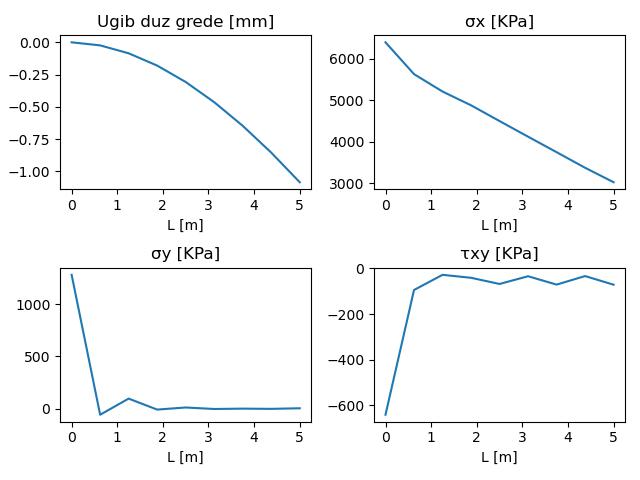
\includegraphics[width=\textwidth]{Slike/Rezultat_4KE.png}
\caption{Python - 4 KE}
\end{figure}
\newpage
Резултат скрипте за мрежу од 16 коначних елемента:
\begin{figure}[H]
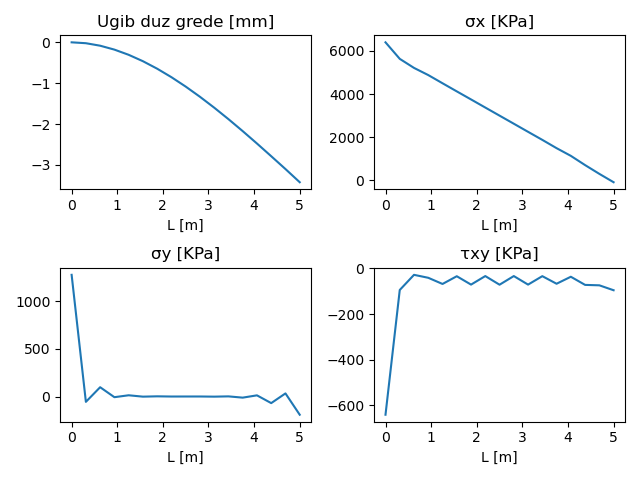
\includegraphics[width=\textwidth]{Slike/Rezultat_16KE.png}
\caption{Python - 16 KE}
\end{figure}
За греду из SAP-а  која је моделирана као танка плоча напрегнута у својој равни (plate-thin) резултати су следећи:
\begin{figure}[H]
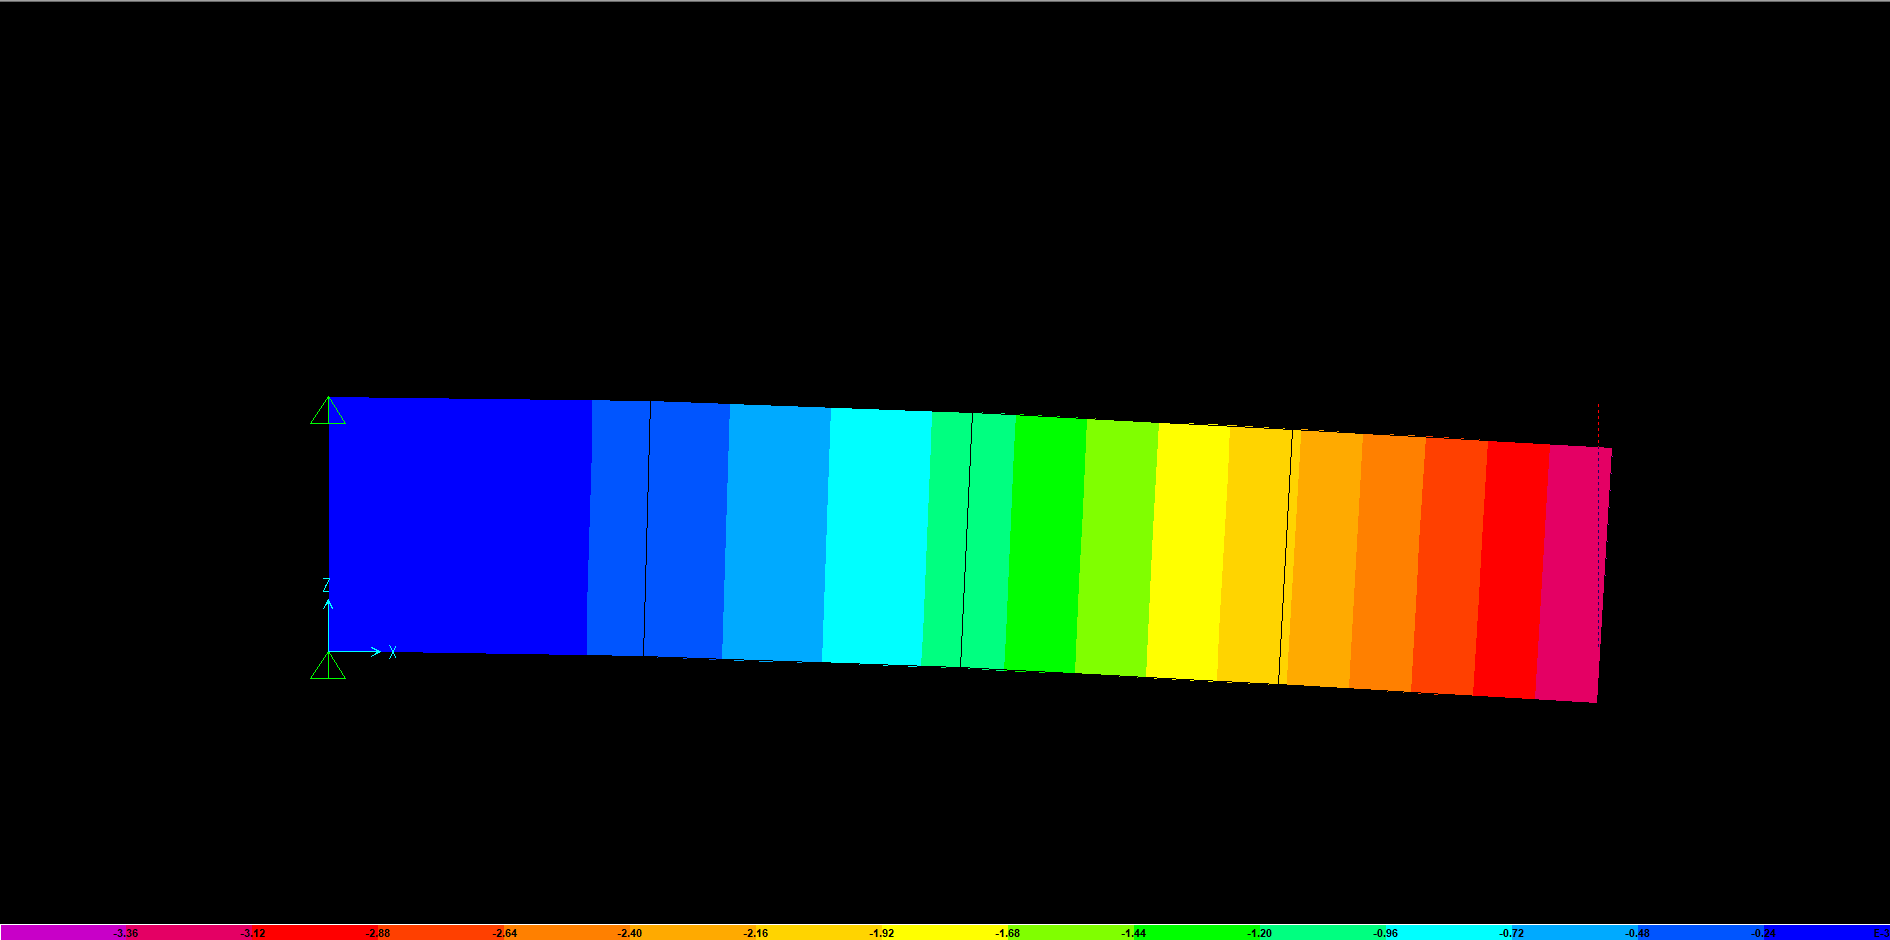
\includegraphics[width=\textwidth]{Slike/Ugib_4KE.png}
\caption{Ugib - 4 KE}
\end{figure}
\begin{figure}[H]
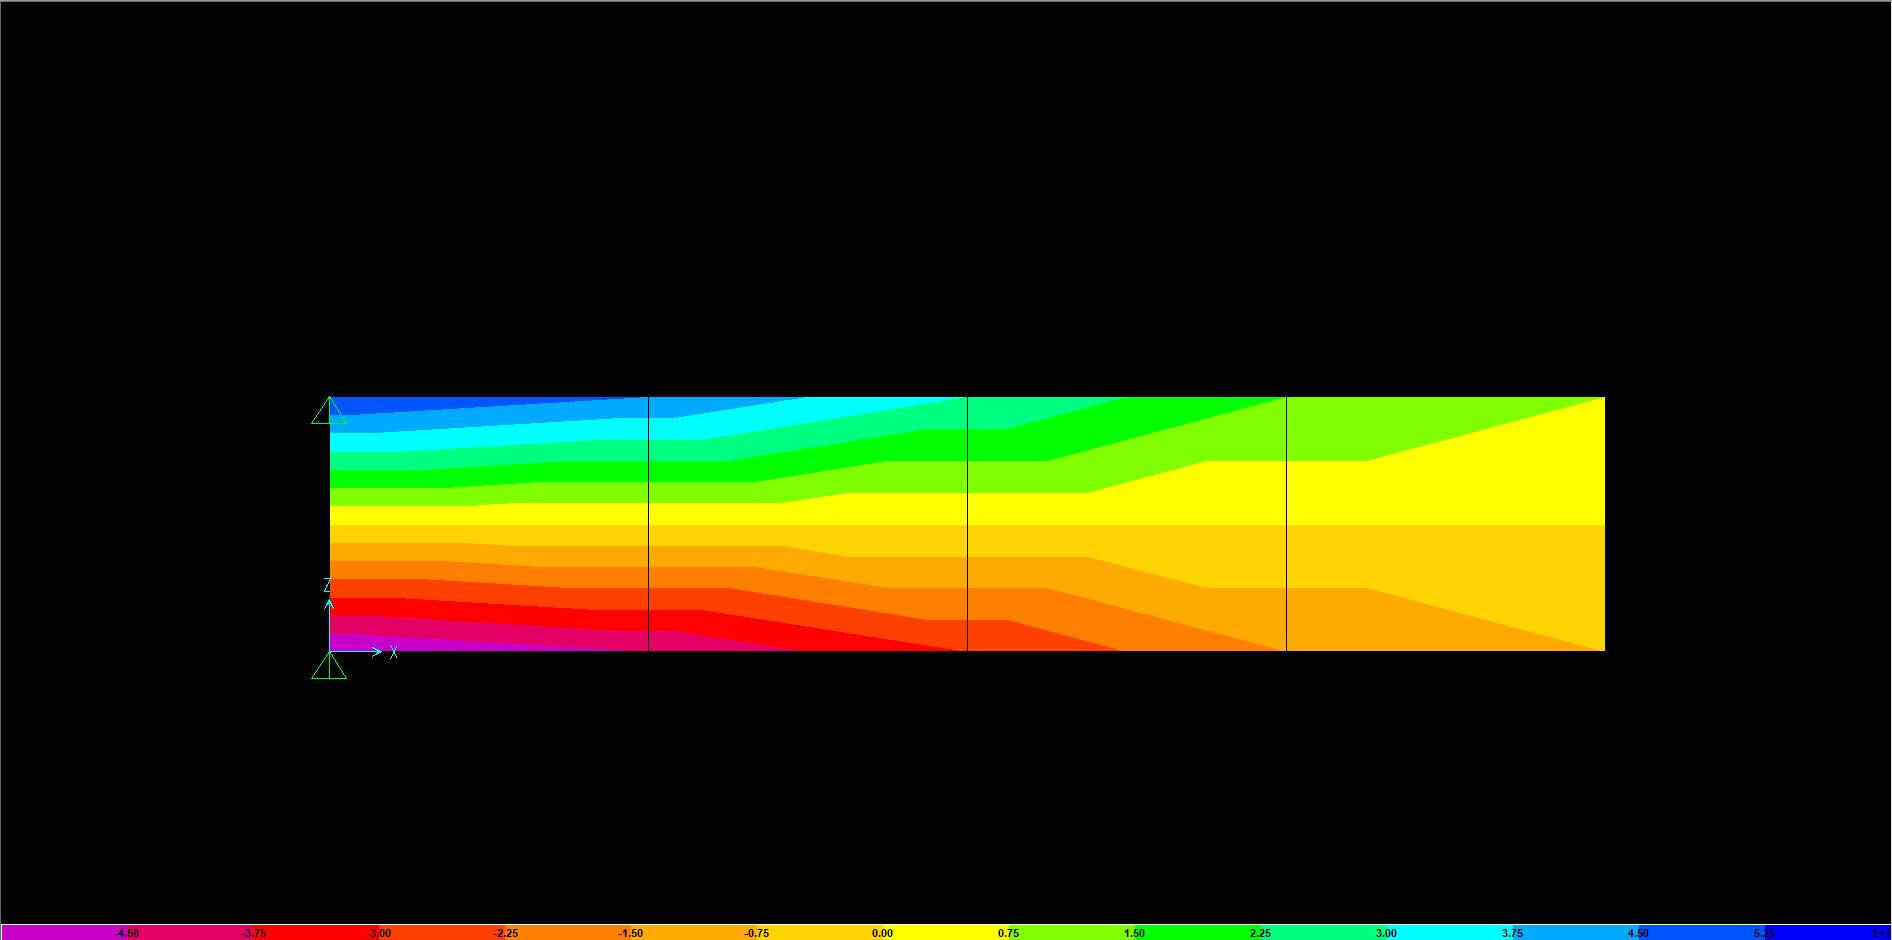
\includegraphics[width=\textwidth]{Slike/Naponi_4KE.png}
\caption{Napon $\sigma_x$ - 4 KE}
\end{figure}
\begin{figure}[H]
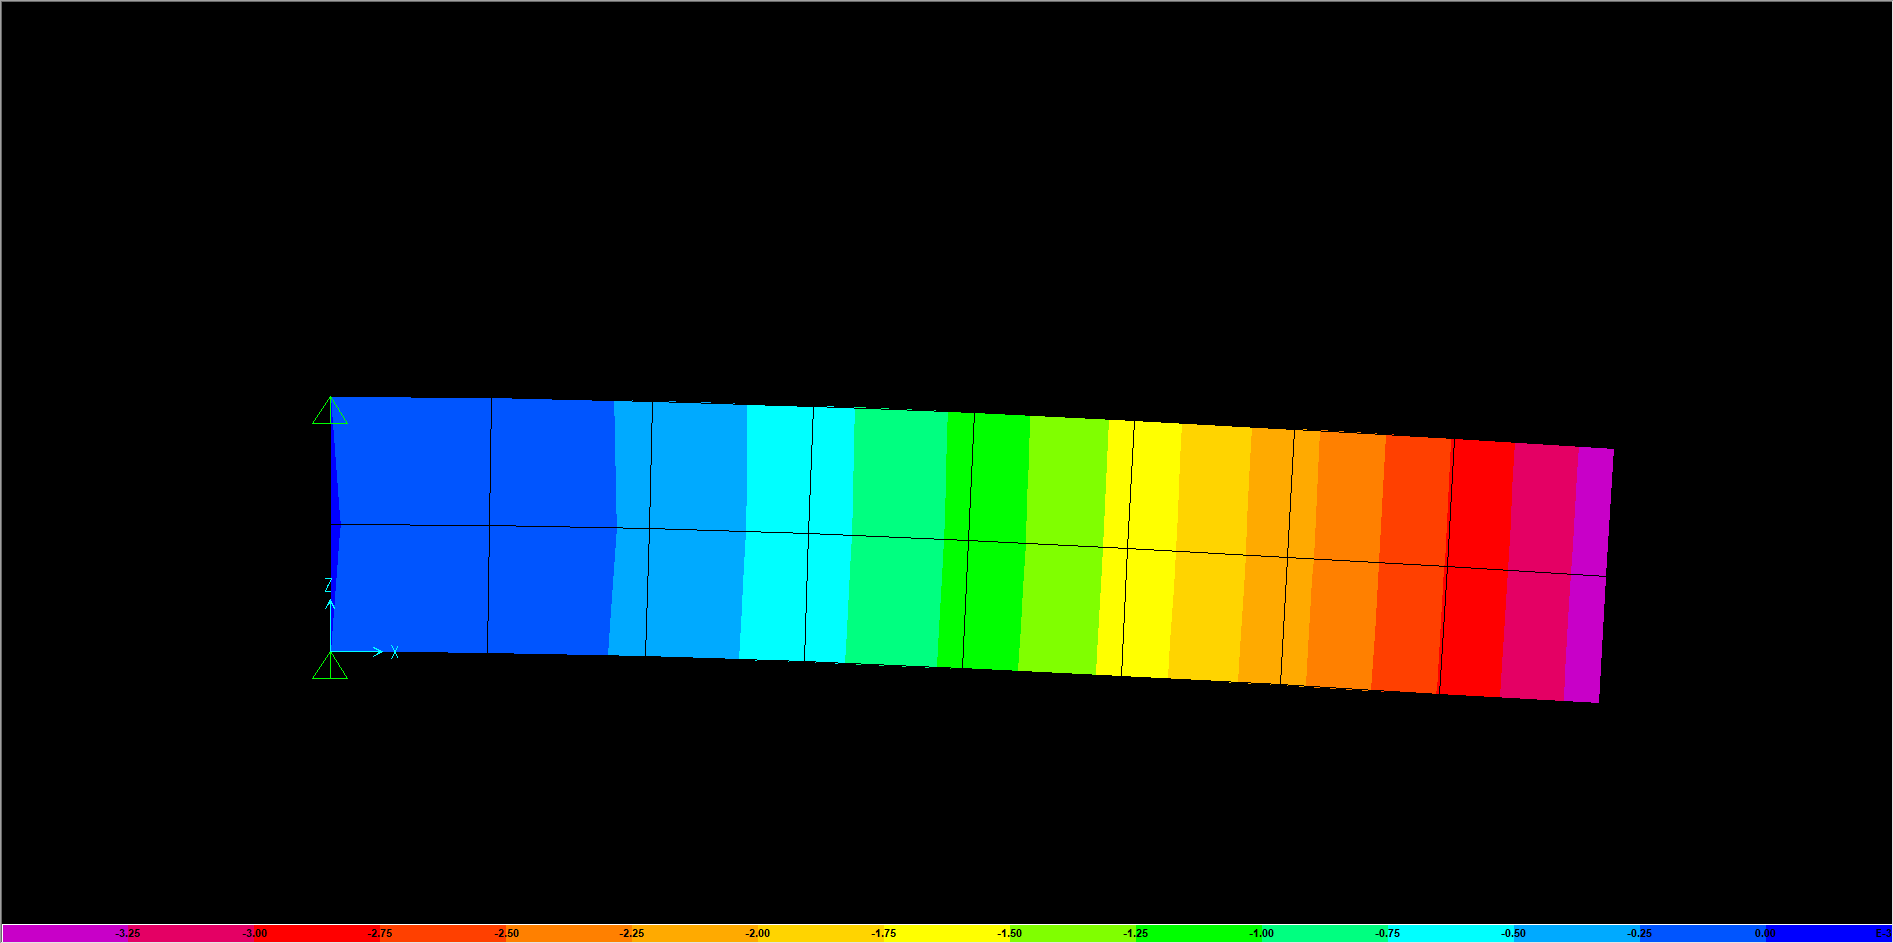
\includegraphics[width=\textwidth]{Slike/Ugib_16KE.png}
\caption{Ugib - 16 KE}
\end{figure}
\begin{figure}[H]
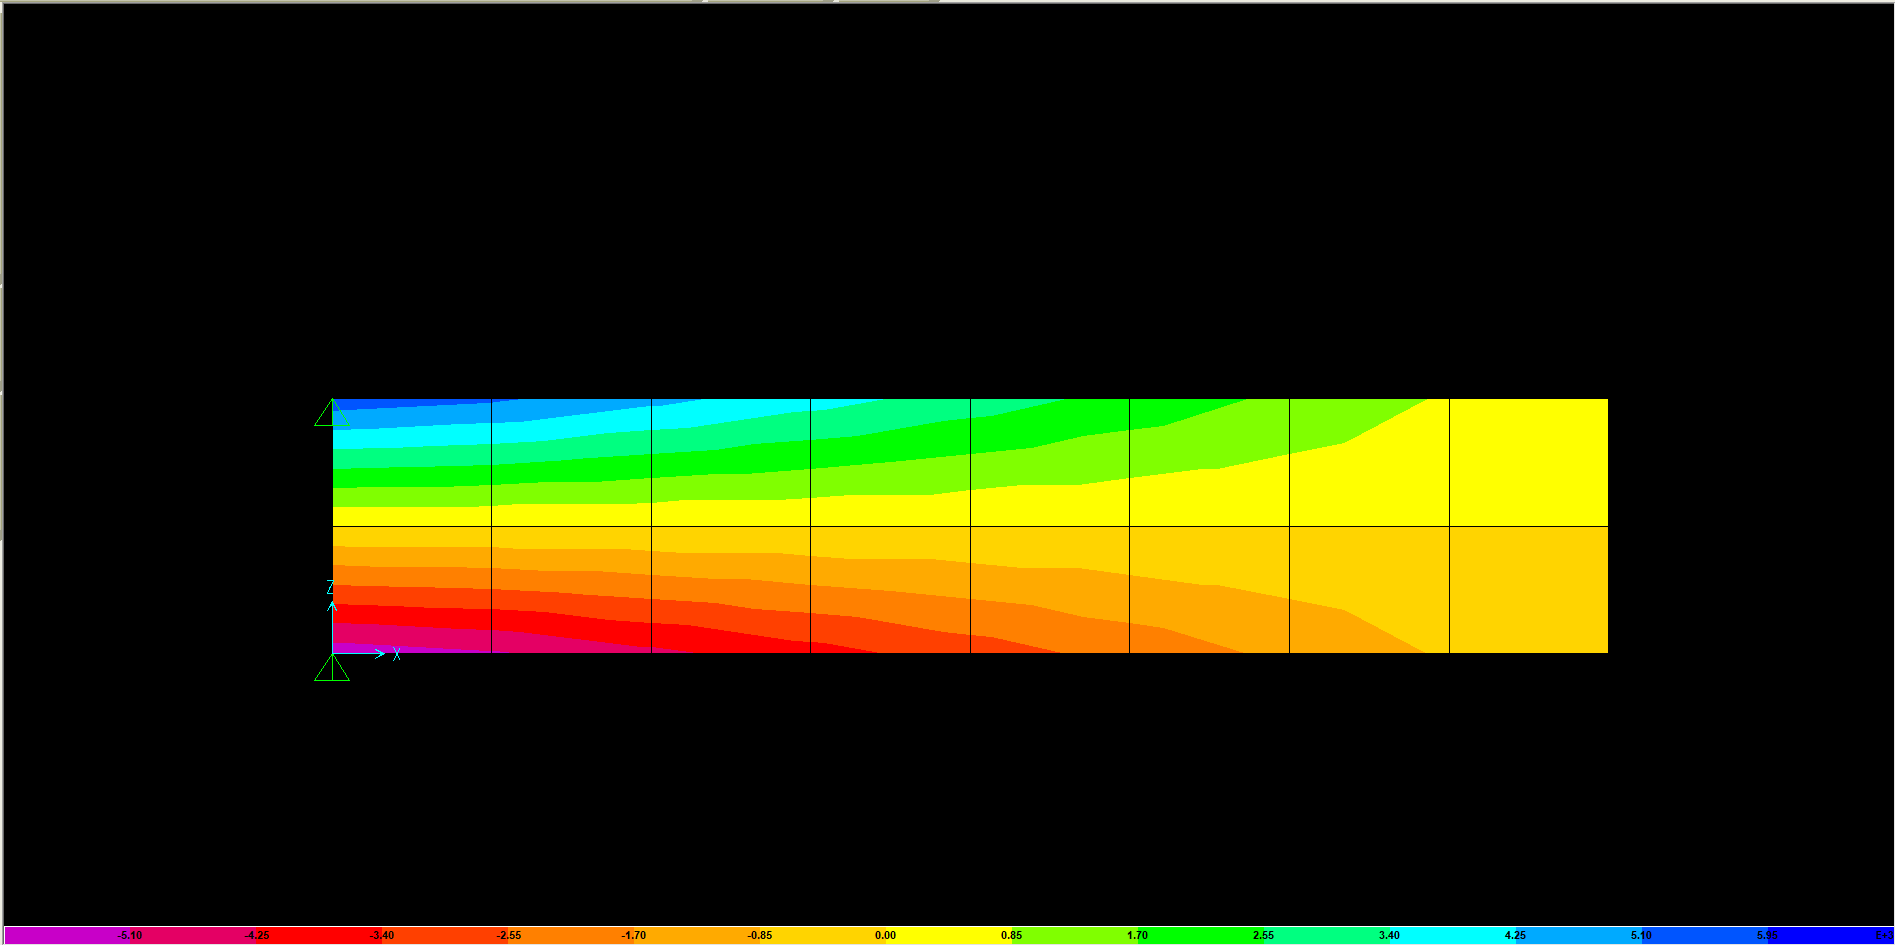
\includegraphics[width=\textwidth]{Slike/Naponi_16KE.png}
\caption{Napon $\sigma_x$ - 16 KE}
\end{figure}
На основу приказаних резултата се може приметити да модел са Q9 коначним елементима има веће деформације од модела из SAP-a који примењује Q4 коначне елементе из чега се може закључити да је матрица крутости Q9 коначног елемента нешто флексибилнија од Q4 коначног елемента. Резултати су врло блиски са аналитичким решењем уколико се примени гушћа мрежа, мрежа са 4 коначна елемента даје приближне вредности напона али далеко непрецизније вредности угиба дуж греде па је потребно прогустити мрежу приликом примене Q9 коначних елемената.
\newpage
\section{Трећи задатак}
\subsection{Диспозиција и информације о параметрима}
За континуални носач приказан на следећој слици је потребно варирати односе $H/L$ и $c/L$ и на основу добијених резултата донети закључке:
\begin{figure}[H]
	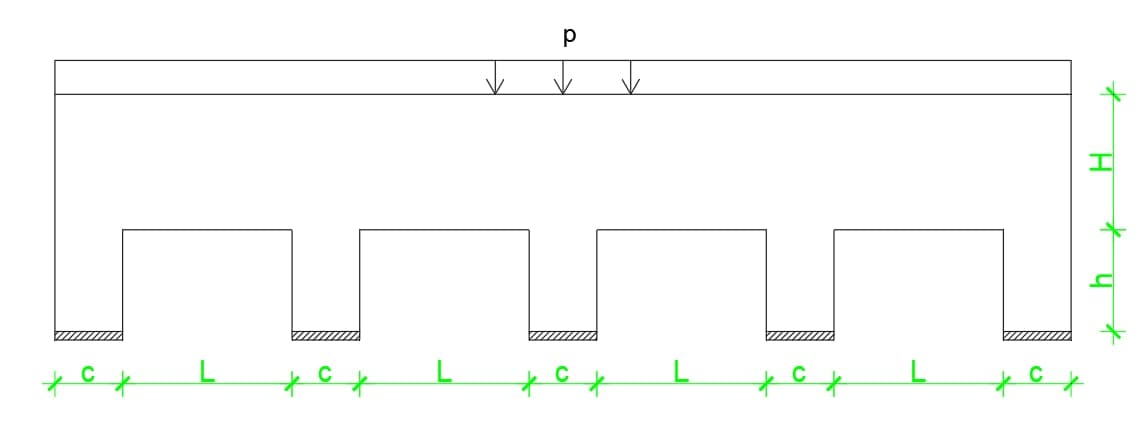
\includegraphics[width=\textwidth, height=5cm]{Slike/Dispozicija.jpg}
	\caption{Диспозиција континуалног носача}
\end{figure}
Параметри који су непроменљиви за све моделе су оптерећење $p=100 kN/m$, дебљина плоче (греде) $d_{pl} = 30cm$ и висина стубова $h=2m$.

\subsection{Дијаграми пресечних сила Nx у зависности од односа димензија}

Резултати су добијени у софтверском пакету Tower demo. Варирањем односа $c/L$ и $H/L$ су приказани следећи резултати:
\newpage
\begin{figure}[H]
	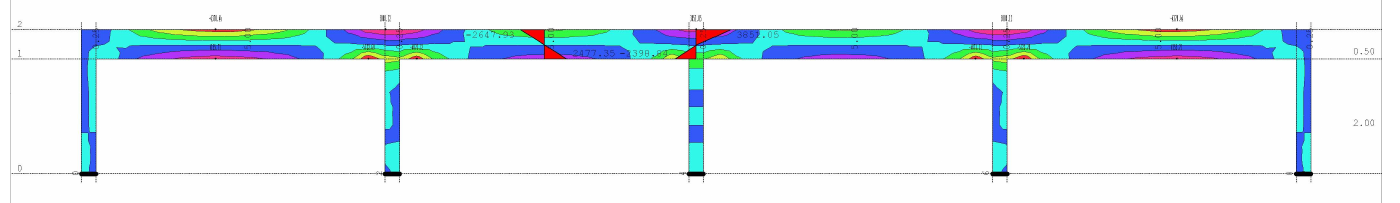
\includegraphics[width=\textwidth, height=7cm]{Slike/C-L_0-05 (0-1).png}
	\caption{c/L=0.05, H/L=0.1}
\end{figure}

\begin{figure}[H]
	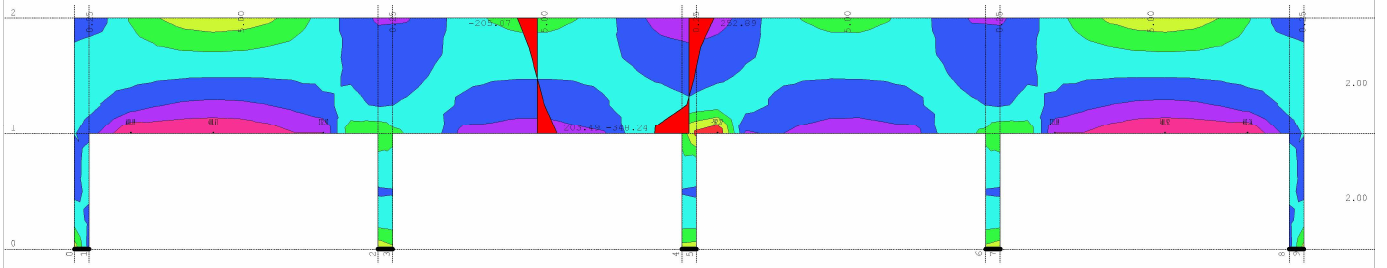
\includegraphics[width=\textwidth, height=7cm]{Slike/C-L_0-05 (0-4).png}
	\caption{c/L=0.05, H/L=0.4}
\end{figure}

\begin{figure}[H]
	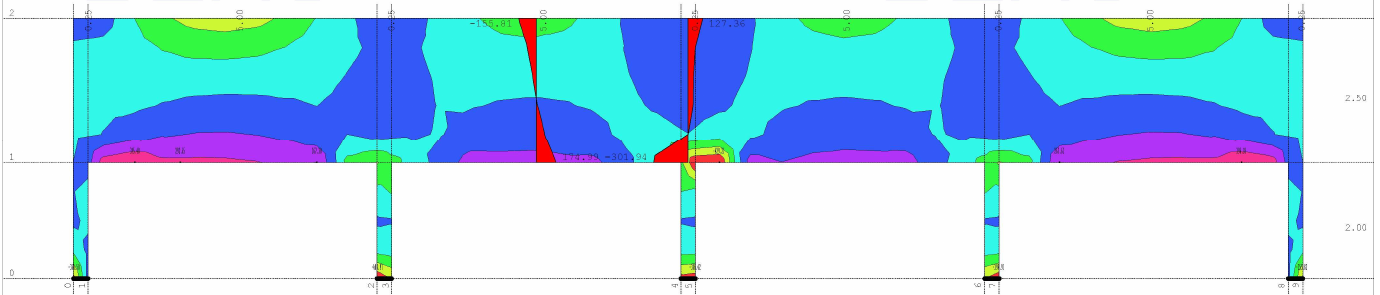
\includegraphics[width=\textwidth, height=7cm]{Slike/C-L_0-05 (0-5).png}
	\caption{c/L=0.05, H/L=0.5}
\end{figure}
\newpage
\begin{figure}[H]
	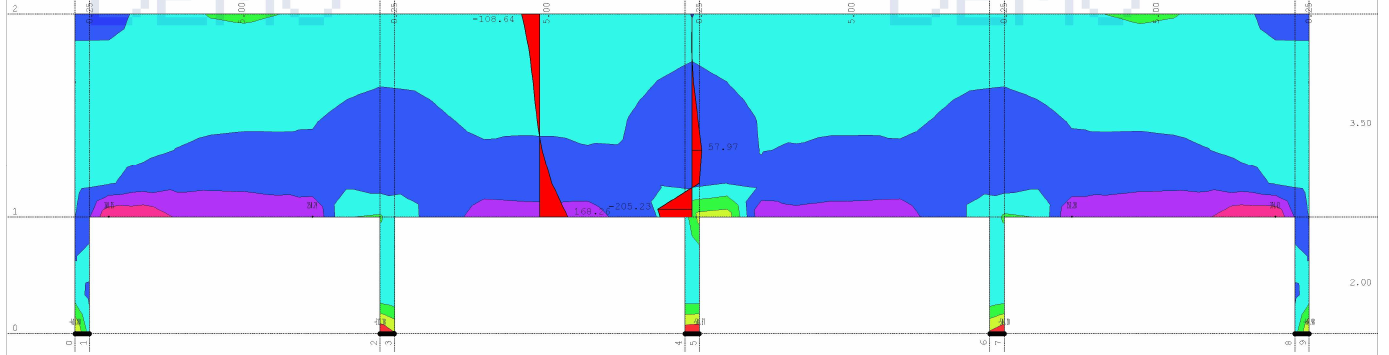
\includegraphics[width=\textwidth, height=7cm]{Slike/C-L_0-05 (0-7).png}
	\caption{c/L=0.05, H/L=0.7}
\end{figure}

\begin{figure}[H]
	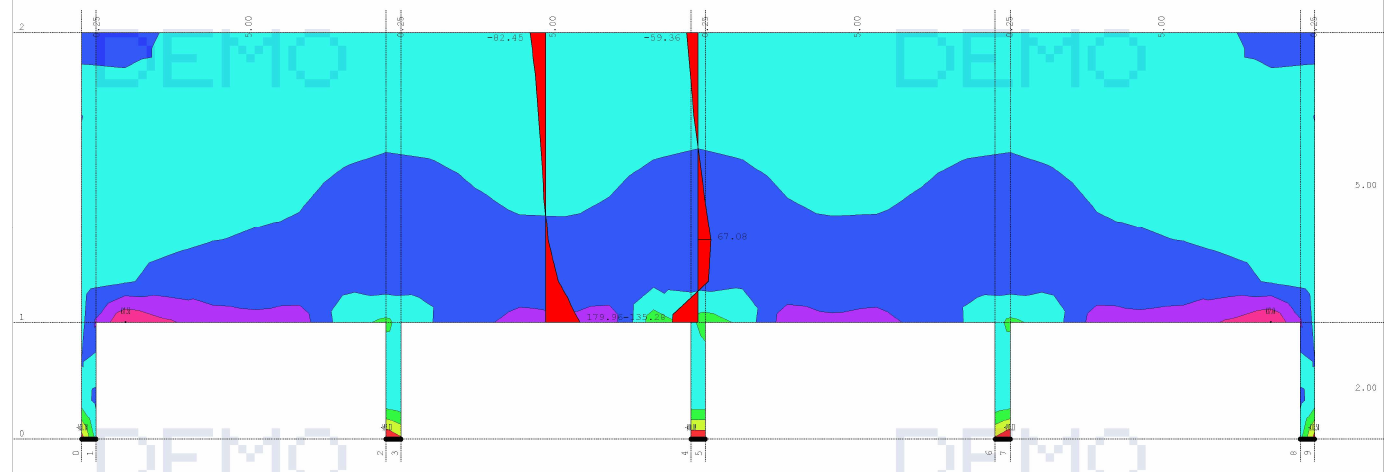
\includegraphics[width=\textwidth, height=7cm]{Slike/C-L_0-05 (1-0).png}
	\caption{c/L=0.05, H/L=1}
\end{figure}

\begin{figure}[H]
	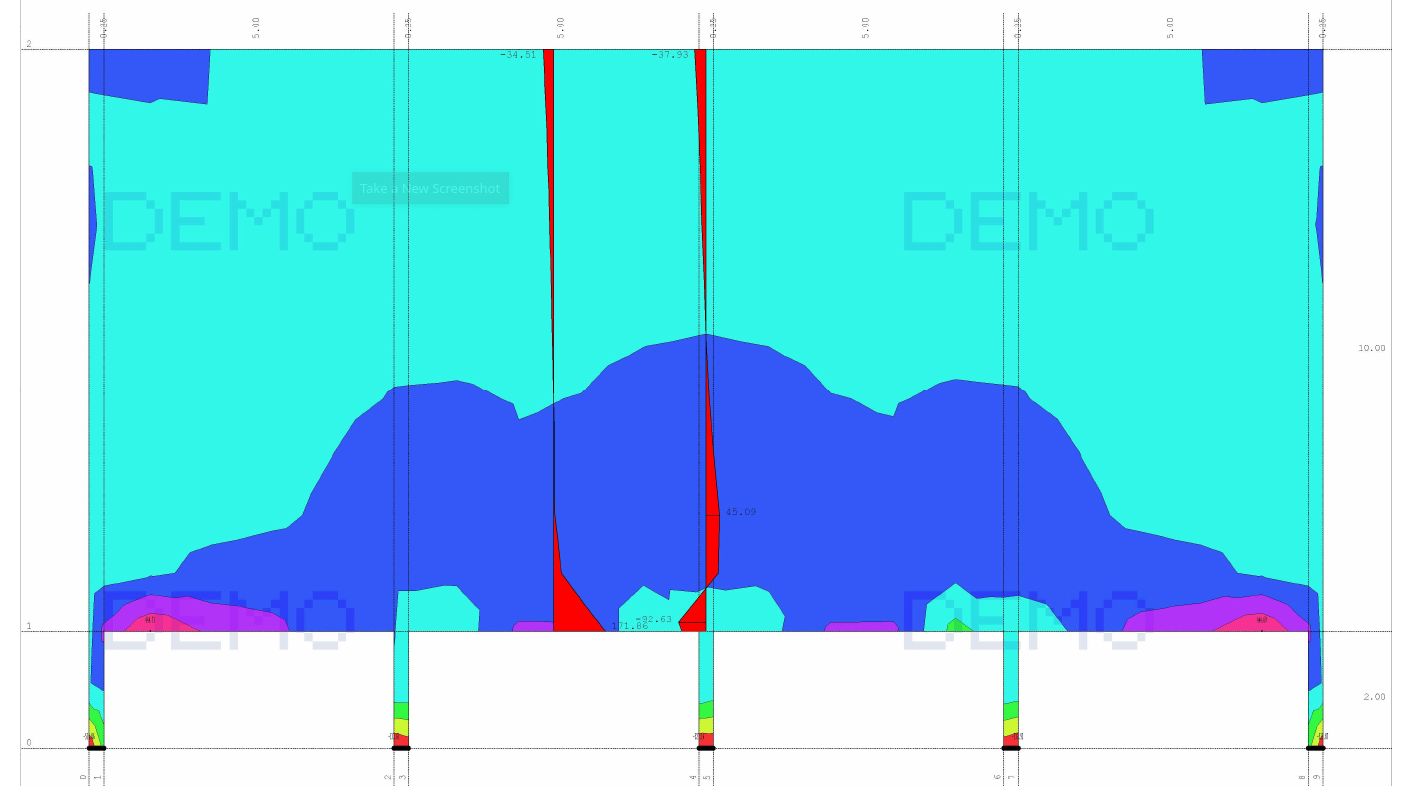
\includegraphics[width=\textwidth, height=7cm]{Slike/C-L_0-05 (2-0).png}
	\caption{c/L=0.05, H/L=2}
\end{figure}

\begin{figure}[H]
	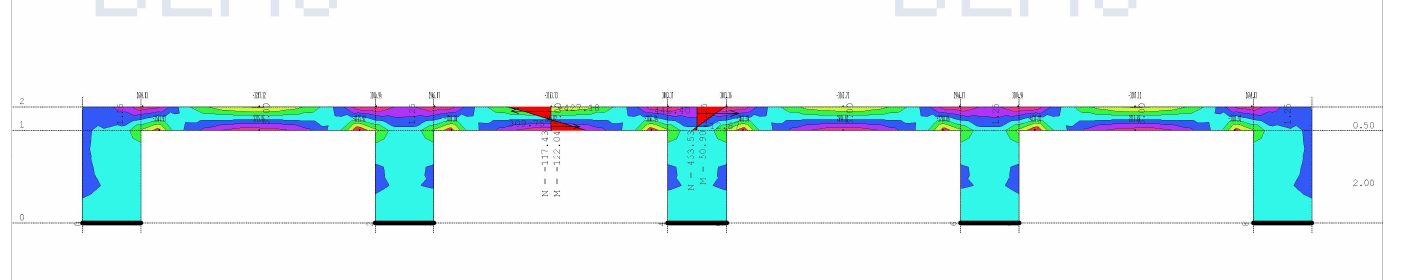
\includegraphics[width=\textwidth, height=7cm]{Slike/C-L_0-25 (0-1).png}
	\caption{c/L=0.25, H/L=0.1}
\end{figure}

\begin{figure}[H]
	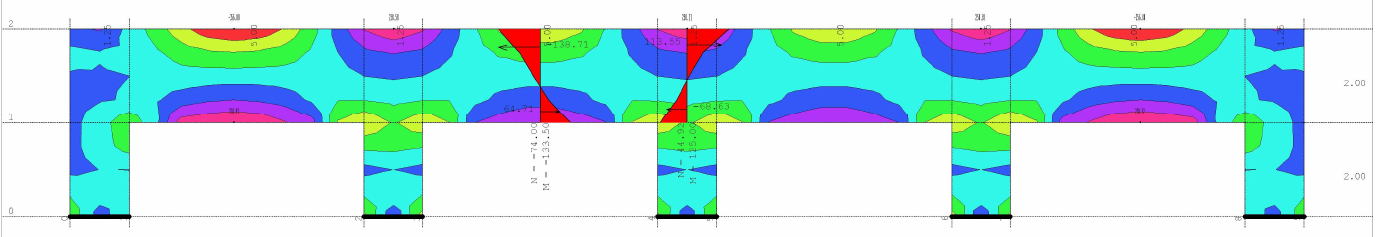
\includegraphics[width=\textwidth, height=7cm]{Slike/C-L_0-25 (0-4).png}
	\caption{c/L=0.25, H/L=0.4}
\end{figure}

\begin{figure}[H]
	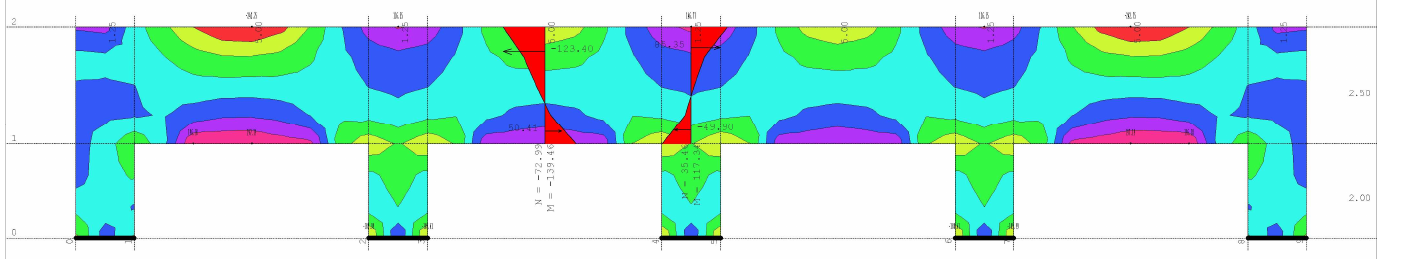
\includegraphics[width=\textwidth, height=7cm]{Slike/C-L_0-25 (0-5).png}
	\caption{c/L=0.25, H/L=0.5}
\end{figure}
\newpage
\begin{figure}[H]
	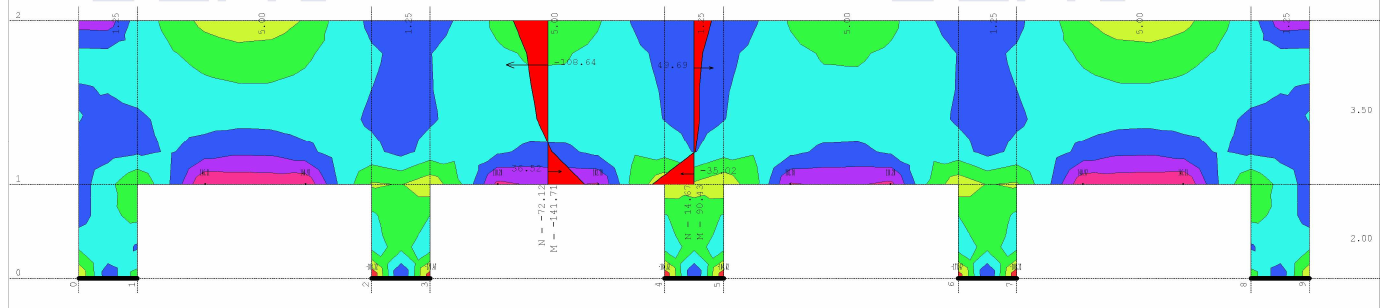
\includegraphics[width=\textwidth, height=7cm]{Slike/C-L_0-25 (0-7).png}
	\caption{c/L=0.25, H/L=0.7}
\end{figure}

\begin{figure}[H]
	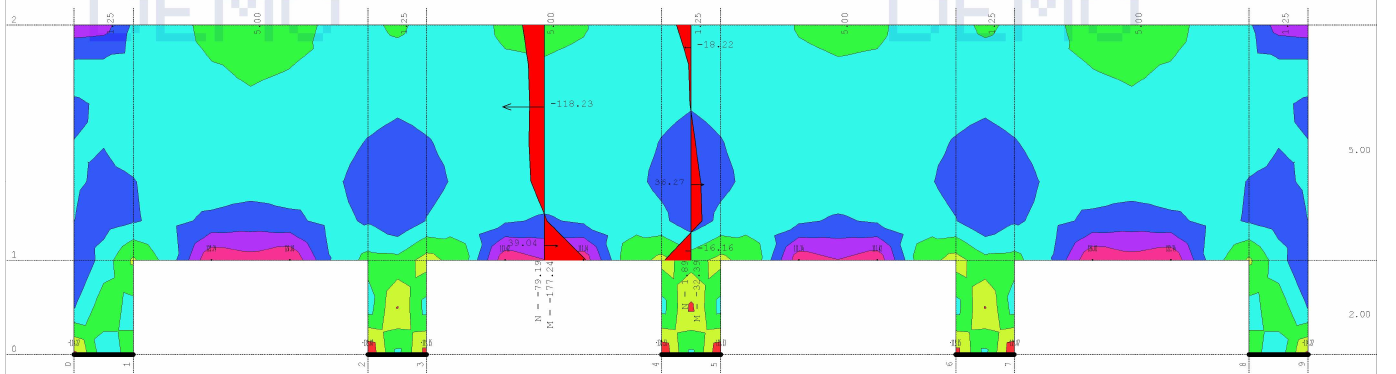
\includegraphics[width=\textwidth, height=7cm]{Slike/C-L_0-25 (1-0).png}
	\caption{c/L=0.25, H/L=1}
\end{figure}

\begin{figure}[H]
	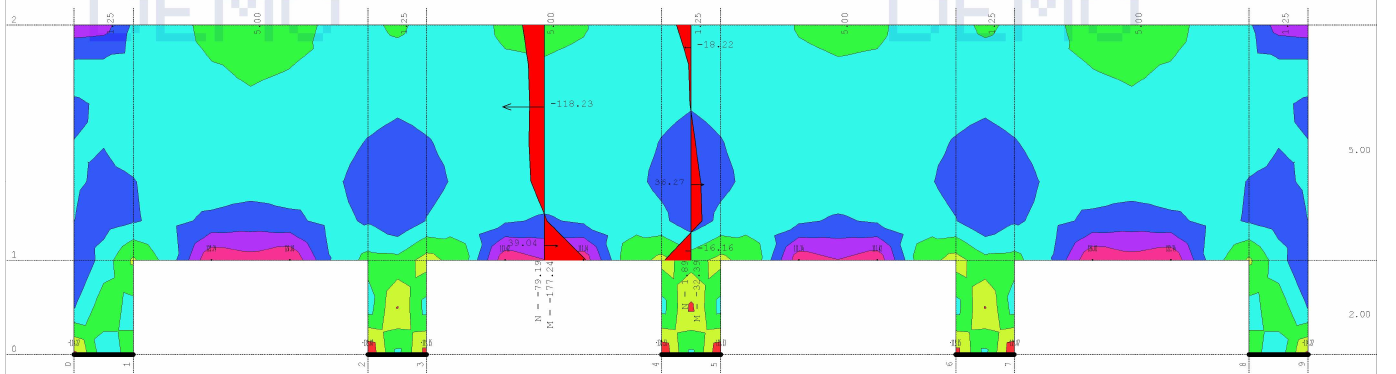
\includegraphics[width=\textwidth, height=7cm]{Slike/C-L_0-25 (1-0).png}
	\caption{c/L=0.25, H/L=2}
\end{figure}
\newpage
\begin{figure}[H]
	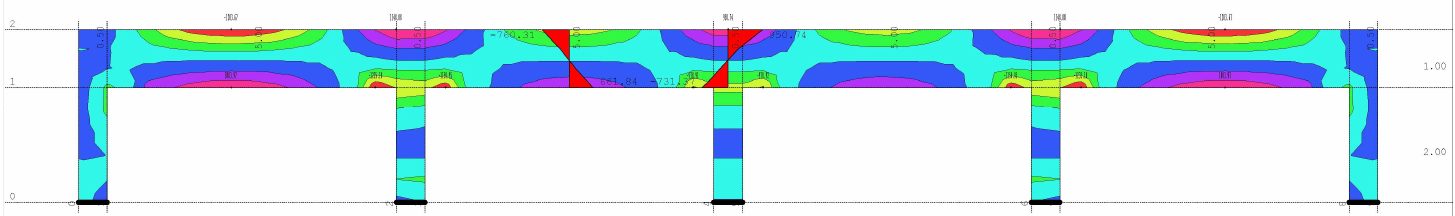
\includegraphics[width=\textwidth, height=7cm]{Slike/H-L_0-2 (0-1).png}
	\caption{H/L=0.2, c/L=0.1}
\end{figure}

\begin{figure}[H]
	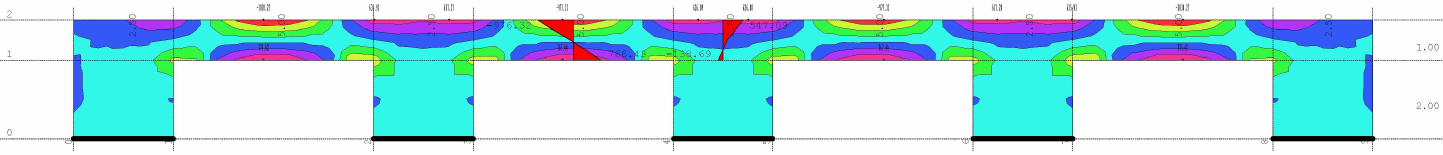
\includegraphics[width=\textwidth, height=7cm]{Slike/H-L_0-2 (0-5).png}
	\caption{H/L=0.2, c/L=0.5}
\end{figure}

\begin{figure}[H]
	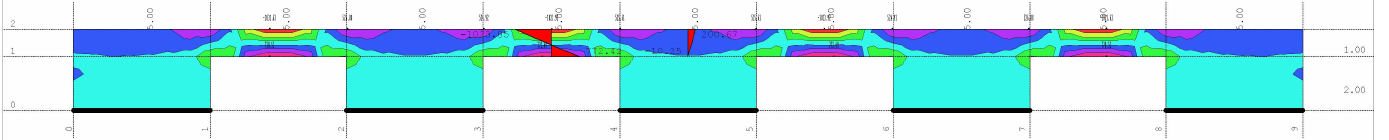
\includegraphics[width=\textwidth, height=7cm]{Slike/H-L_0-2 (1-0).png}
	\caption{H/L=0.2, c/L=1}
\end{figure}
\newpage
\begin{figure}[H]
	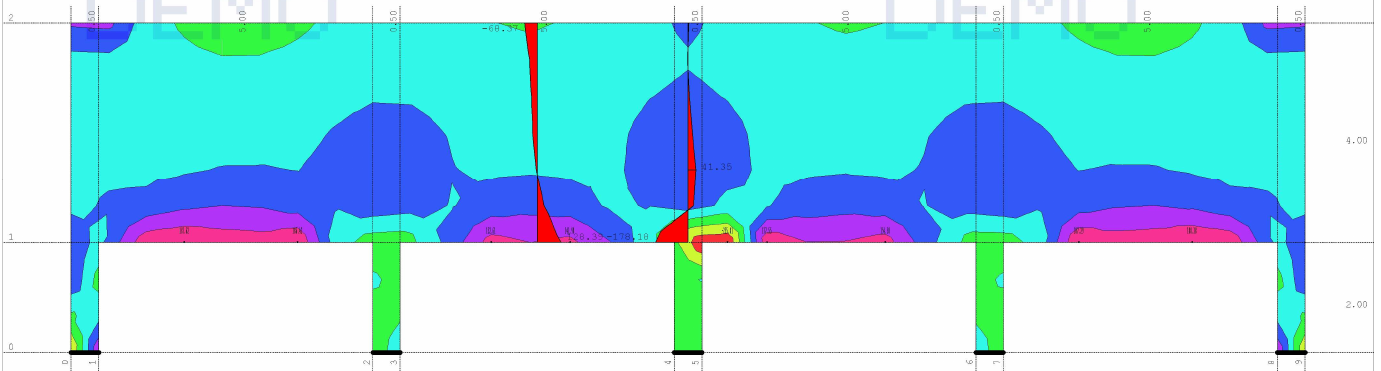
\includegraphics[width=\textwidth, height=7cm]{Slike/H-L_0-8 (0-1).png}
	\caption{H/L=0.8, c/L=0.1}
\end{figure}

\begin{figure}[H]
	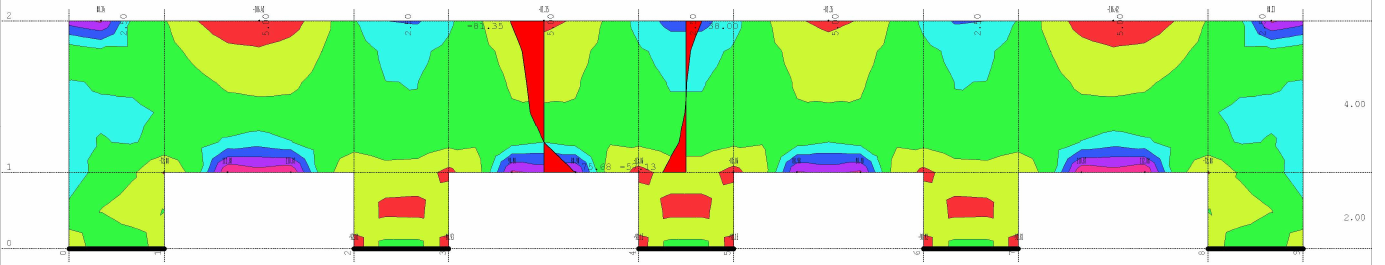
\includegraphics[width=\textwidth, height=7cm]{Slike/H-L_0-8 (0-5).png}
	\caption{H/L=0.8, c/L=0.5}
\end{figure}

\begin{figure}[H]
	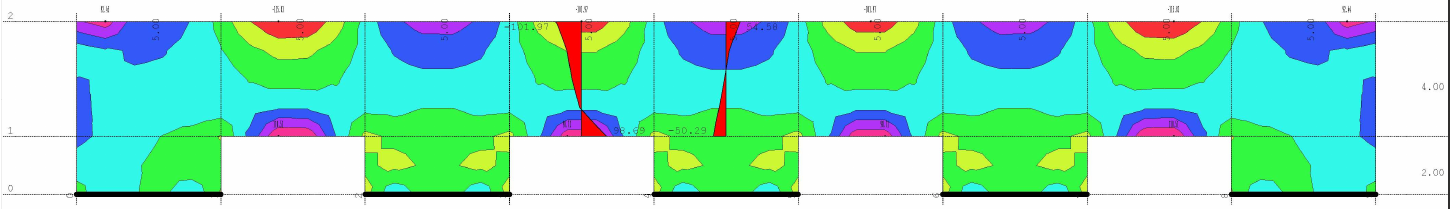
\includegraphics[width=\textwidth, height=7cm]{Slike/H-L_0-8 (1-0).png}
	\caption{H/L=0.8, c/L=1}
\end{figure}
\newpage
\begin{figure}[H]
	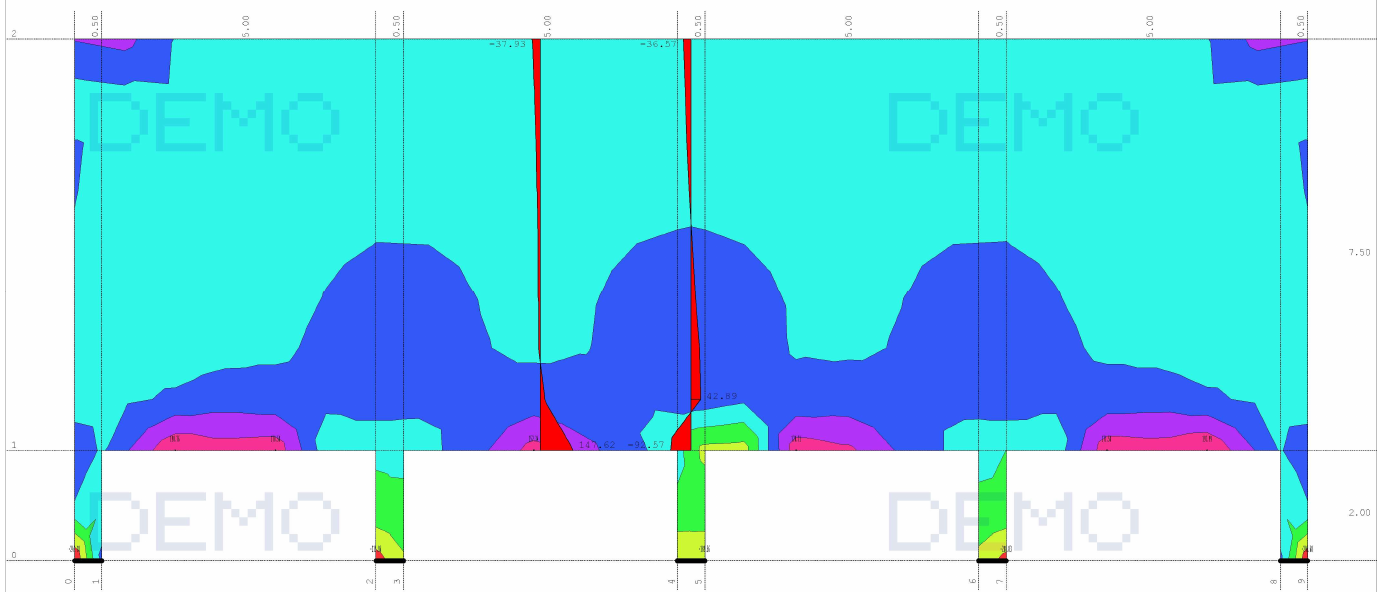
\includegraphics[width=\textwidth, height=7cm]{Slike/H-L_1-5 (0-1).png}
	\caption{H/L=1.5, c/L=0.1}
\end{figure}

\begin{figure}[H]
	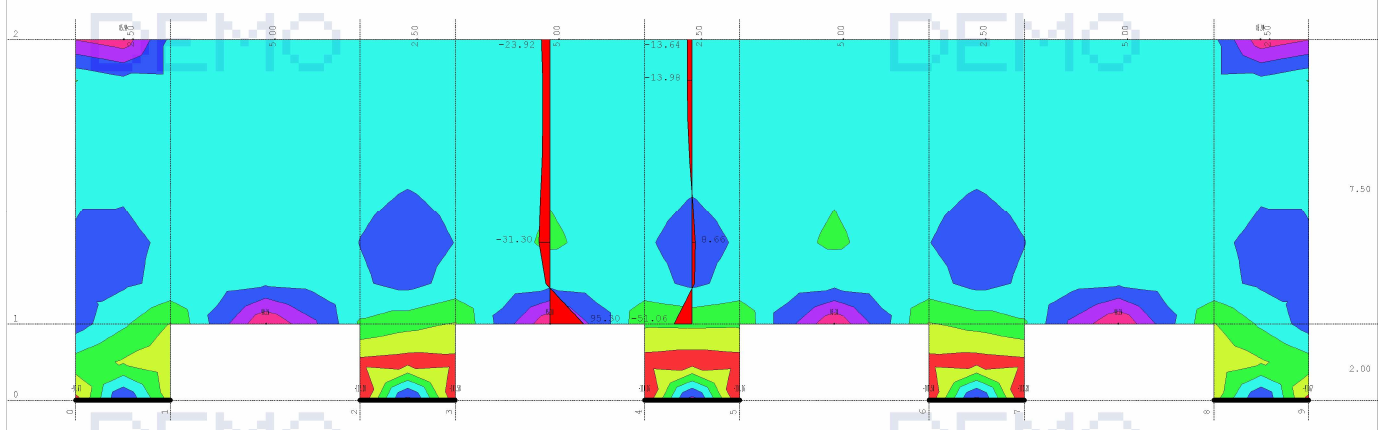
\includegraphics[width=\textwidth, height=7cm]{Slike/H-L_1-5 (0-5).png}
	\caption{H/L=1.5, c/L=0.5}
\end{figure}

\begin{figure}[H]
	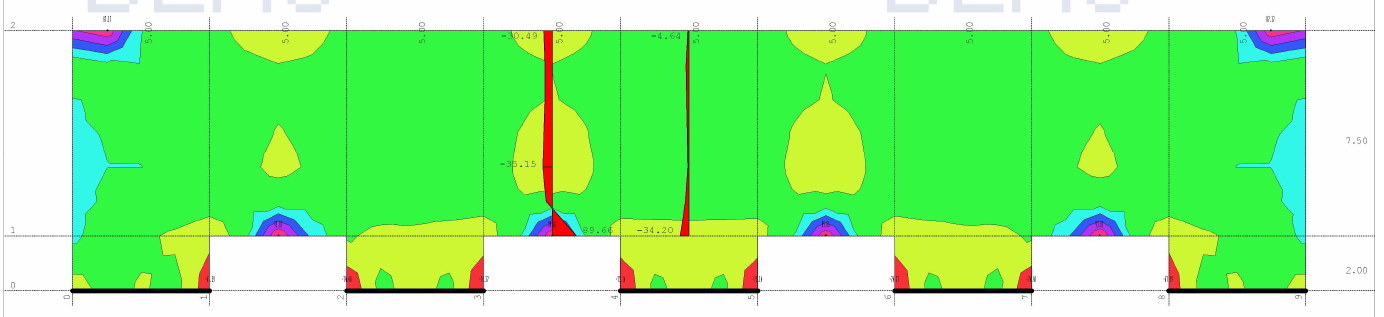
\includegraphics[width=\textwidth, height=7cm]{Slike/H-L_1-5 (1-0).png}
	\caption{H/L=1.5, c/L=1}
\end{figure}

Табеларни приказ пресечних сила у пољу и над ослонцем за горње и доње влакно са графицима за различите фиксне односе $c/L$ и варирањем $H/L$:


\begin{figure}[H]
	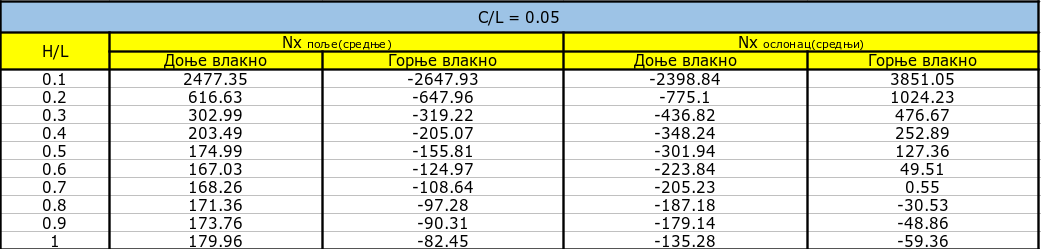
\includegraphics[width=\textwidth, height=6cm]{Slike/Tabela_0.05.png}
	\caption{Промена пресечних сила $N_x$ варирањем односа $H/L$ за фиксни однос $c/L = 0.05$}
\end{figure}

\begin{figure}[H]
	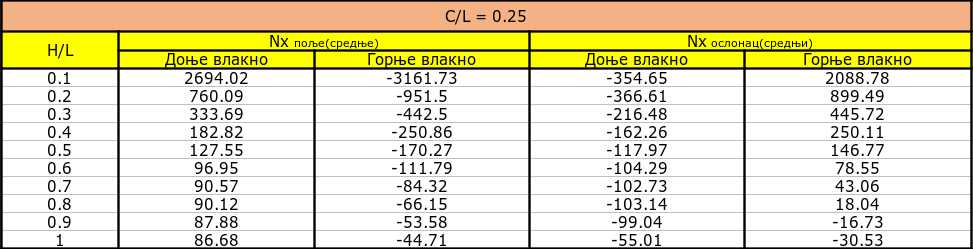
\includegraphics[width=\textwidth, height=6cm]{Slike/Tabela_0.25.png}
	\caption{Промена пресечних сила $N_x$ варирањем односа $H/L$ за фиксни однос $c/L = 0.25$}
\end{figure}

\begin{figure}[H]
	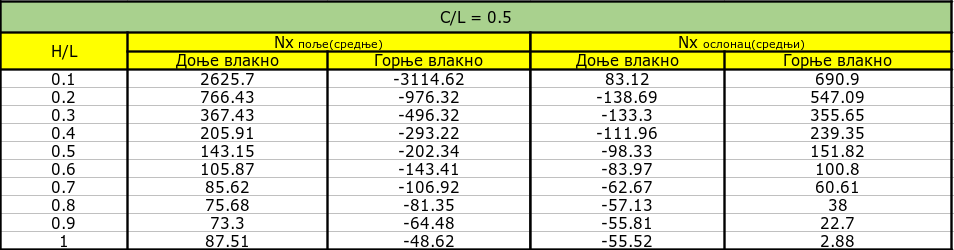
\includegraphics[width=\textwidth, height=6cm]{Slike/Tabela_0.5.png}
	\caption{Промена пресечних сила $N_x$ варирањем односа $H/L$ за фиксни однос $c/L = 0.5$}
\end{figure}

\begin{figure}[H]
	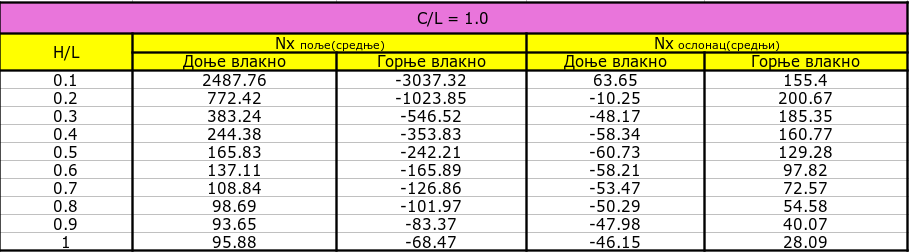
\includegraphics[width=\textwidth, height=6cm]{Slike/Tabela_1.png}
	\caption{Промена пресечних сила $N_x$ варирањем односа $H/L$ за фиксни однос $c/L =1$}
\end{figure}

\begin{figure}[H]
	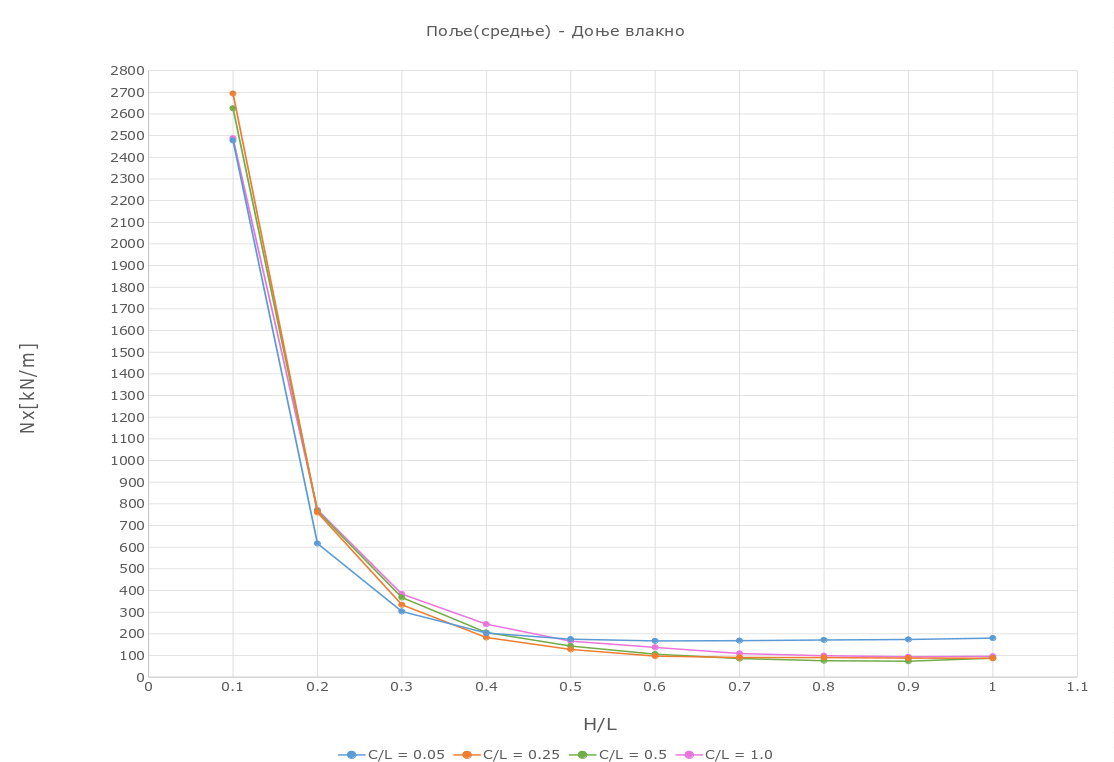
\includegraphics[width=\textwidth, height=10cm]{Slike/Polje_donje.png}
	\caption{График промене пресечних сила $N_x$ доњег влакна у средњем пољу}
\end{figure}

\begin{figure}[H]
	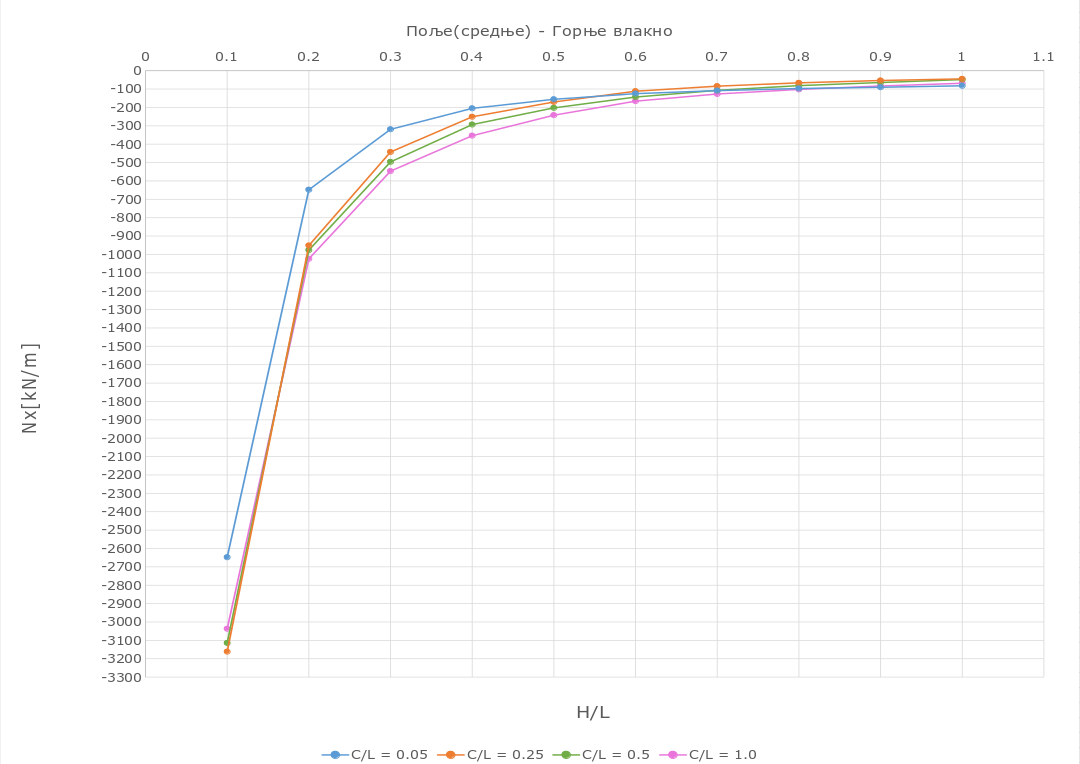
\includegraphics[width=\textwidth, height=10cm]{Slike/Polje_gornje.png}
	\caption{График промене пресечних сила $N_x$ горњег влакна у средњем пољу}
\end{figure}

\begin{figure}[H]
	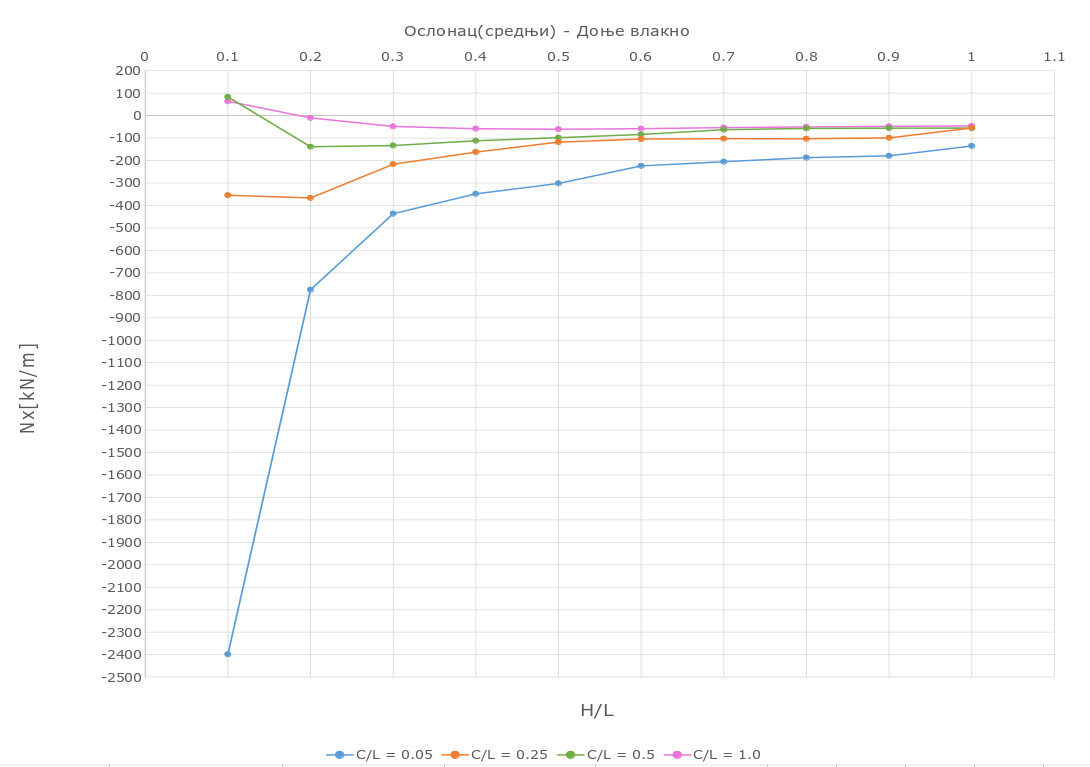
\includegraphics[width=\textwidth, height=10cm]{Slike/Oslonac_donje.png}
	\caption{График промене пресечних сила $N_x$ доњег влакна над средњим ослонцем}
\end{figure}

\begin{figure}[H]
	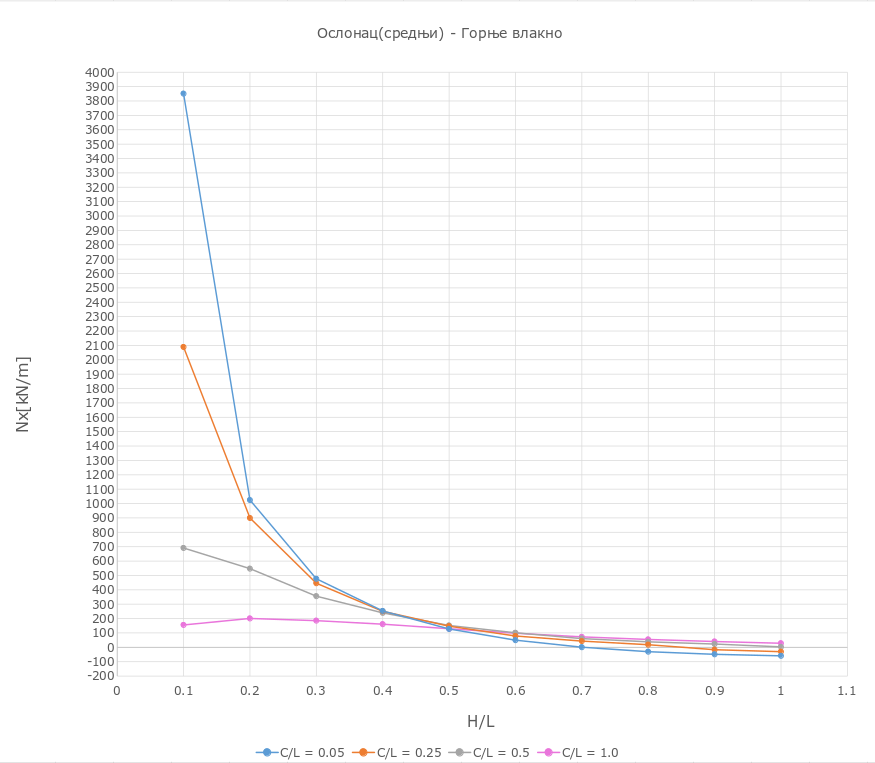
\includegraphics[width=\textwidth, height=10cm]{Slike/Oslonac_gornje.png}
	\caption{График промене пресечних сила $N_x$ горњег влакна над средњим ослонцем}
\end{figure}


\subsection{Закључак}
Због ограничења Tower верзије могућност сагледавања резултата је за мрежу од максимално 300 чворова коначних елемената.\\
Пресечне силе у средњем пољу континуалног носача не одступају превише од свог "симетричног" понашања за горње и доње влакно за исту вредност $c/L$ као ни пресечне силе над ослонцем, међутим повећавањем односа $c/L$ се вредност пресечне силе $N_x$ смањује што указује на изражену крутост стубова на савијање који на себе прикупљају утицаје момената па и утицај са тиме опада у два пресека. За мали однос $c/L$ стубови се понашају као прости штапови па нису у могућности да на себе "навуку" додатне утицаје. 
На дијаграмима се такође види да повећањем односа $H/L$ носач почиње да се понаша као зидни носач због расподеле пресечних сила по висини пресека која више није линеарна за разлику од мањих односа $H/L$ који одговара више гредним носачима.
\newpage
\section{Прилози}
Упутство за инсталирање Python-a и потребних пакета можете пронаћи на:
\url{https://codeberg.org/nikolal/VKMKE}\\
Кратку документацију са описима рада метода можете пронаћи на:
\url{https://codeberg.org/nikolal/VKMKE/wiki}\\
Код скрипти можете пронаћи на следећим линковима:\\
zad1.py: \url{https://codeberg.org/nikolal/VKMKE/src/branch/master/zad1.py}
zad2.py: \url{https://codeberg.org/nikolal/VKMKE/src/branch/master/zad2.py}\\
mapiranjeQ9.py: \url{https://codeberg.org/nikolal/VKMKE/src/branch/master/mapiranjeQ9.py}
\newpage
\addcontentsline{toc}{section}{Литература}
\printbibliography
\end{document}